\documentclass[12pt,a4paper]{article}
\usepackage[a4paper,margin=2.54cm,headheight=15pt]{geometry}
\usepackage[T1]{fontenc}
\usepackage[utf8]{inputenc}
\usepackage[english]{babel}
\usepackage{amsmath,amsthm,amssymb}
\usepackage{newtxtext,newtxmath}
\usepackage{microtype}
\usepackage[onehalfspacing]{setspace}
\usepackage[parfill]{parskip}
\usepackage{graphicx}
\graphicspath{{images/}}
\usepackage{float}
\usepackage{placeins}
\usepackage{xcolor}
\usepackage{fancyhdr}
\pagestyle{fancy}
\fancyhf{}
\fancyhead[R]{\thepage}
\renewcommand{\headrulewidth}{0pt}
\usepackage{titlesec}
\setcounter{secnumdepth}{3}
\titleformat{\section}{\normalfont\large\bfseries}{\thesection.}{0.6em}{}
\titleformat{\subsection}{\normalfont\normalsize\bfseries}{\thesubsection}{0.9em}{}
\titleformat{\subsubsection}{\normalfont\normalsize}{\thesubsubsection}{0.9em}{}
\titlespacing*{\section}{0pt}{18pt}{10pt}
\titlespacing*{\subsection}{1.2em}{14pt}{8pt}
\titlespacing*{\subsubsection}{2.6em}{12pt}{6pt}
\usepackage{tocloft}
\setcounter{tocdepth}{3}
\addto\captionsenglish{\renewcommand{\contentsname}{Table of Contents}}
\tocloftpagestyle{fancy}
\renewcommand{\cfttoctitlefont}{\large\bfseries}
\renewcommand{\cftsecaftersnum}{.}
\renewcommand{\cftsecfont}{\bfseries\itshape}
\renewcommand{\cftsecpagefont}{\bfseries\itshape}
\renewcommand{\cftsecleader}{\cftdotfill{\cftdotsep}}
\renewcommand{\cftsubsecfont}{\bfseries}
\renewcommand{\cftsubsecpagefont}{\bfseries}
\usepackage{caption}
\definecolor{captionblue}{RGB}{47,84,150}
\captionsetup[figure]{labelsep=period,
  justification=raggedright,singlelinecheck=false,
  font={small}}
\usepackage{listings}
\definecolor{codebg}{RGB}{245,245,245}
\definecolor{mlkeyword}{RGB}{14,0,255}
\definecolor{mlcomment}{RGB}{2,128,9}
\definecolor{mlstring}{RGB}{170,4,249}
\lstdefinestyle{matlabcode}{
  language=Matlab,
  basicstyle=\footnotesize\ttfamily\linespread{1.0}\selectfont,
  keywordstyle=\color{mlkeyword},
  commentstyle=\color{mlcomment},
  stringstyle=\color{mlstring},
  backgroundcolor=\color{codebg},
  showstringspaces=false,
  breaklines=true,
  keepspaces=true,
  columns=fullflexible,
  aboveskip=8pt,belowskip=8pt,
  xleftmargin=4pt,xrightmargin=4pt,
  framesep=4pt,frame=single,rulecolor=\color{codebg}}
\lstnewenvironment{matlab}{\lstset{style=matlabcode}}{}
\newcommand{\labfigure}[3][0.85\textwidth]{%
  \begin{figure}[H]
    \centering
    \includegraphics[width=#1]{#2}
    \caption{}\label{#3}
  \end{figure}}
\newcommand{\figref}[1]{Figure~\ref{#1}}
\newcommand{\codeused}[1][]{\par\textbf{Code used#1:}\par\vspace{-4pt}}
\newcommand{\templateused}[1][]{\par\textbf{Template used#1:}\par\vspace{-4pt}}
\newcommand{\hx}{\texorpdfstring{\,\texttimes\,}{x}}
\usepackage[breaklinks=true,colorlinks=true,linkcolor=blue,urlcolor=blue,citecolor=blue,unicode]{hyperref}
\hypersetup{%
  bookmarksopen = true,
  pdfauthor     = {Egor Chumakov},
  pdftitle      = {Egor Chumakov -- Digital Signal Processing 2 Lab Diary},
  pdfsubject    = {Laboratory protocols -- FH Salzburg}}
\begin{document}
\begin{titlepage}
  \centering

  
\includegraphics[width=2.4cm]{fhs_logo.pdf}

  \vspace*{1.5cm}

  {\Large\bfseries Digital Signal Processing 2}

  \vspace*{1.5cm}

  {\large Laboratory protocols,\\
   including homework assignments}

  \vfill

  Egor Chumakov -- 2510721013\\
  \href{mailto:fhs54864@fh-salzburg.ac.at}{fhs54864@fh-salzburg.ac.at}

  \vspace*{0.8cm}

  Salzburg, 16 July 2026

  \vspace*{1cm}
\end{titlepage}

\setcounter{page}{2}
\tableofcontents

% =====================================================================
%  LAB 1 -- FIR und IIR Filter Design
%  Headings copied word for word from DSP2_Lab1.pdf
% =====================================================================
\clearpage
\section{Lab exercise 1: FIR und IIR Filter Design}

% ---------------------------------------------------------------------
% Like in the DSP1 diary, each chapter starts with your own theory
% introduction (about one page) before the first subsection.
% ---------------------------------------------------------------------
TODO: chapter introduction -- theory about FIR and IIR filters, window
method, equiripple method, that will be followed in the laboratory work.

\subsection{Laboratory 1 -- The task is to compare FIR Filters with different windows and to implement an own IIR filter function.}

\subsubsection{(a) Use the functions developed in the last semester to analyze the audio file ps.wav to determine which noise signal is present.}

TODO

\subsubsection{(b) Experiment with the fdatool (rectangle window) and create a FIR filter that is able to remove the interference from the audio file.}

TODO

\subsubsection{(c) Export the filter using the File/Export menu and filter the audio file. Analyze the result visually in the frequency spectrum as well as aural.}

TODO

\subsubsection{(d) Use different windows for designing the FIR filter and compare the results and explain the advantages and disadvantages. Compare the different filters with the fvtool or with the freqz function}

TODO

\subsubsection{(e) Construct the FIR filter with the Equiripple method. Analyze the differences to the Window method.}

TODO

\subsubsection{(f) Implement your own FIR and IIR filtering function for vector-signals.}

% formula given on the exercise sheet:
\begin{equation}
  y[n] = \sum_{k=1}^{M} b_k \cdot x[n-k] - \sum_{k=1}^{M} a_k \cdot y[n-k]
  \tag{1}
\end{equation}

TODO

\subsubsection{(g) Design with the fdatool an IIR filter which can be used instead of the FIR filter. Export the IIR filter as second-order-sections (SOS).}

TODO

\subsubsection{(h) Implement your own filter function to be able to filter the audio file by using the second-order-sections. Compare the result to the sosfilt function of matlab.}

TODO

\subsection{Homework 1 (Implement your own Overlap-Add FIR-Filter function)}

\subsubsection{Implement your own Overlap-Add FIR-Filter function. Use also your own functions implemented in the winter semester. Compare it with the fftfilt function of matlab.}

TODO

\clearpage
\section{Lab exercise 2: Notch and Comb Filter Design}

Notch filters are used to filter out specific frequency inference with only one specific frequency like 50 or 60 Hz or . Amplitude response has very narrow notch at frequency range to be blocked with other frequencies pass through unchanged. 

Created with second order IIR filter designed directly from pole zero plot so that conjugate complex zero is located at that specific frequency $\omega_{0}$. Since zeros are exactly on the unit circle filter gain at $\omega_{0}$ is zero. For all other frequencies along unit circle distance from zeros and poles is roughly equal so gain is roughly 1. Conjugate complex poles are placed at the same angle but inside the unit circle at distance $r$ from origin with pole radius $r$ controlling steepness and width of the notch. Notch becomes more steep and narrow as r approaches 1. For stability, $r < 1$ must hold.

\begin{figure}[H]
  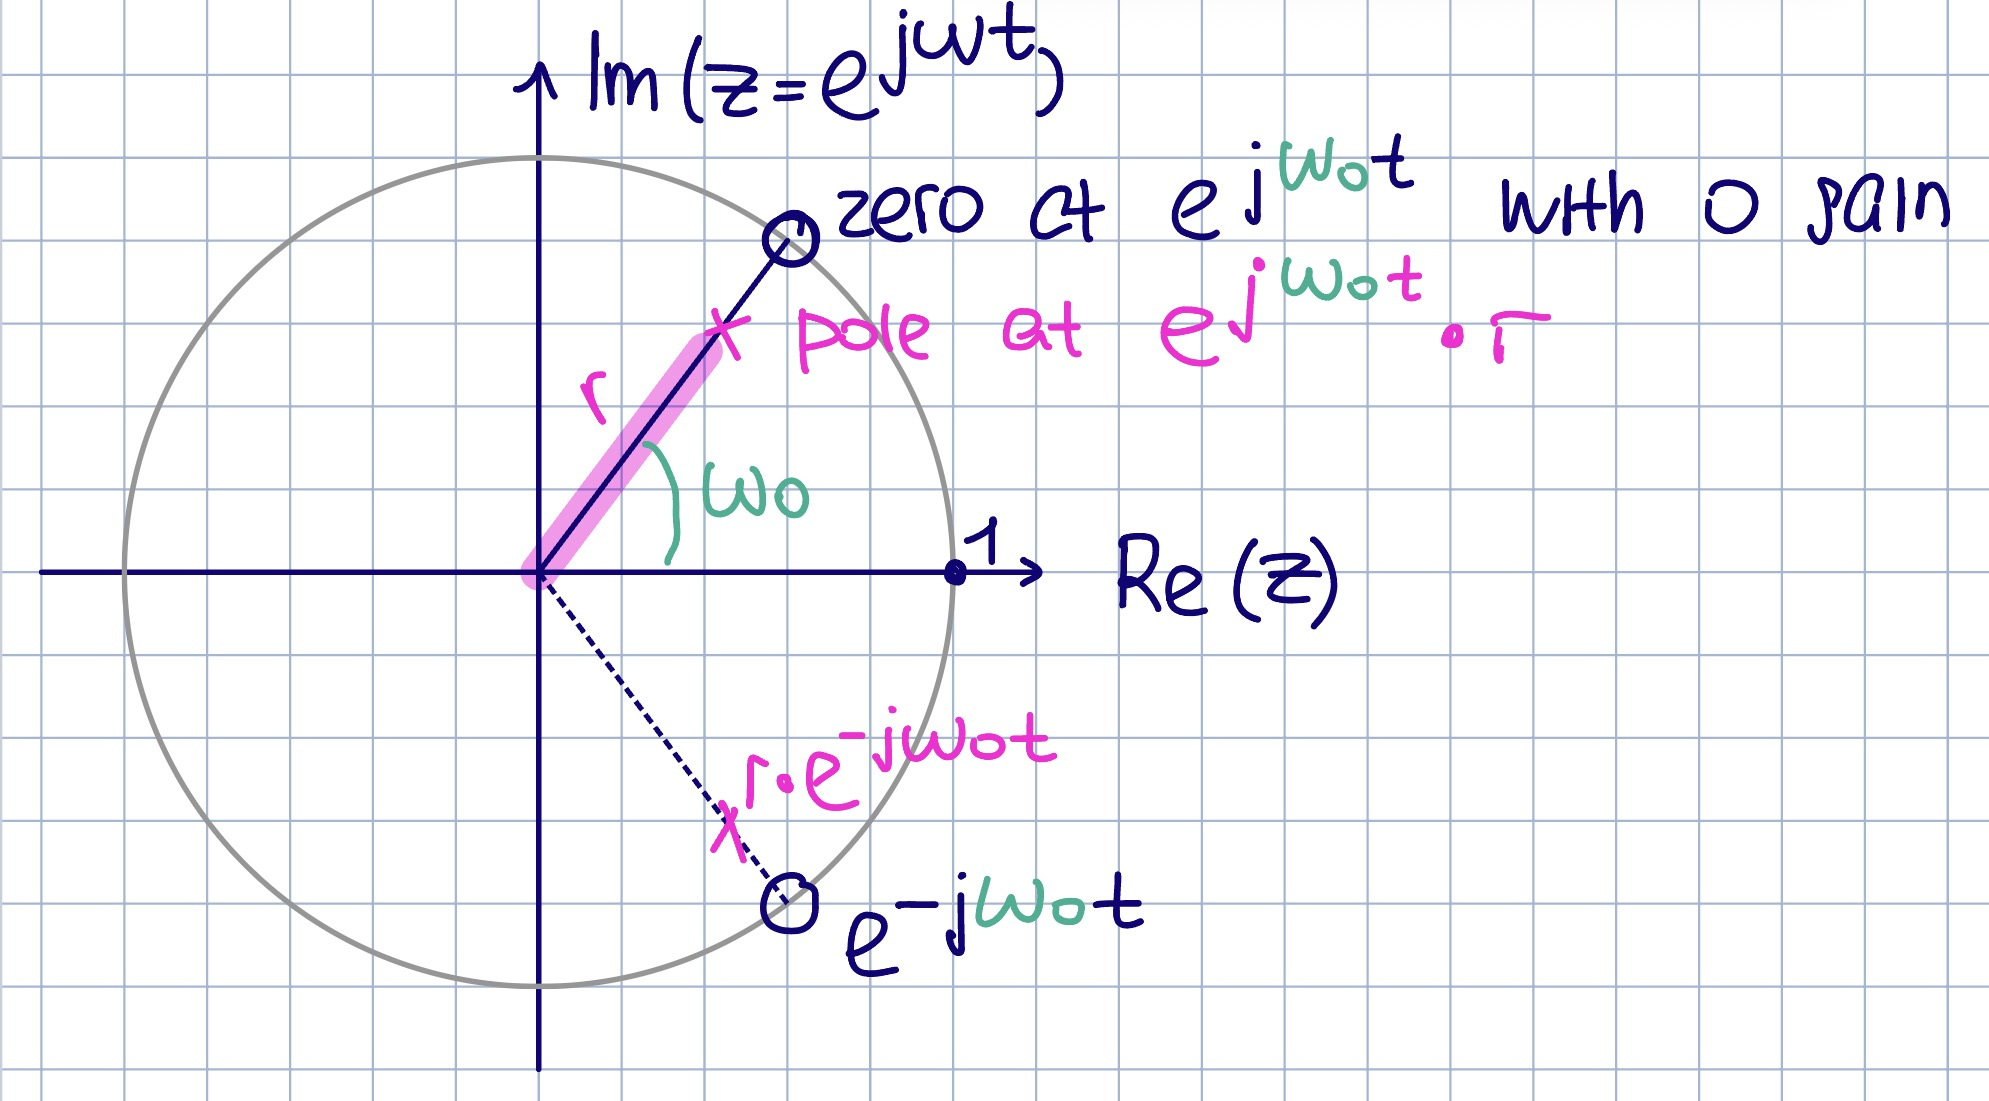
\includegraphics[width=0.6\textwidth]{image_78.png}
  \caption{notch filter pole zero design basic idea}\label{fig:20}
\end{figure}

\subsection{Laboratory 2 -- Design a Notch filter using the Pol-Zero diagram for a stop frequency fs=1000Hz and a sample rate fa=10000Hz. Use as the pole radius r=0.98.}

In transfer function (\ref{eq:notch-tf}) numerator zeros $e^{\pm j\omega_0}$ are on the unit circle and create gain zero at $\omega_0$. Denominator poles $r * e^{\pm j\omega_0}$ are inside the unit circle at radius $r$. Transfer function can be further simplified to form with cosine of angular frequency $\omega_0$ that is used in function for notch filter.

\subsubsection{(a) Write a function to design a Notch filter with the following input parameters:}

% given on the exercise sheet:
\begin{itemize}
  \item stop frequency fs; pole radius r; sampling rate fa
\end{itemize}
With
\begin{equation}
  H(z) = \frac{(z - e^{j\omega_0})(z - e^{-j\omega_0})}
              {(z - re^{j\omega_0})(z - re^{-j\omega_0})}
       = \frac{z^2 - 2z\cos(\omega_0) + 1}
              {z^2 - 2zr\cos(\omega_0) + r^2}
  \label{eq:notch-tf}\tag{1}
\end{equation}
and
\begin{equation}
  \omega_0 = 2\pi\frac{f_s}{f_a}
  \tag{2}
\end{equation}

\begin{figure}[H]
  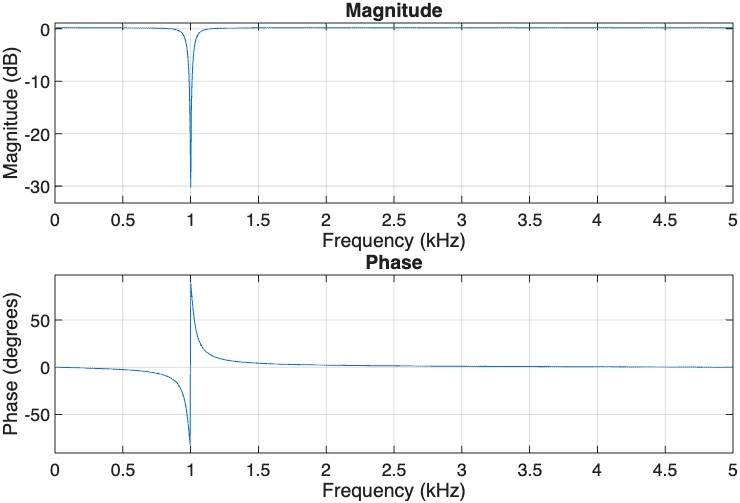
\includegraphics[width=0.48\textwidth]{image_27.jpg}\hspace{4pt}
  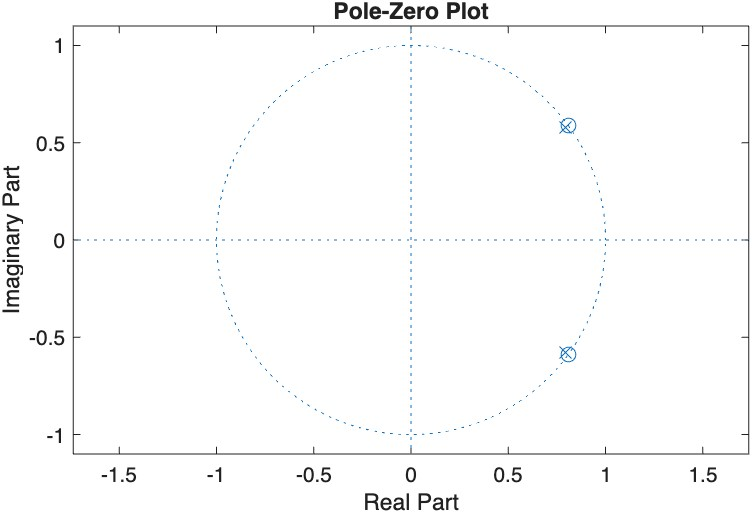
\includegraphics[width=0.48\textwidth]{image_28.jpg}
  \caption{notch filter frequency response and pole-zero map}\label{fig:21}
\end{figure}

notchFilter function computes normalized angular frequency $\omega_0 = 2\pi \cdot f_s / f_a$ and returns numerator coefficients $b$ applied to input and denominator coefficients $a$ from feedback. 

For $f_s = 1000$ Hz, $f_a = 10000$ Hz, $r = 0.98$ output is:

\begin{figure}[H]
  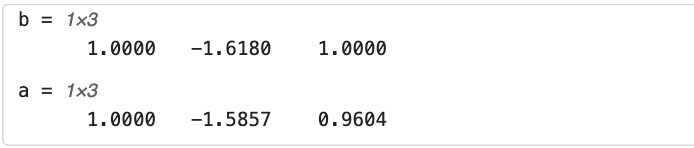
\includegraphics[width=0.6\textwidth]{image_79.png}
  \caption{notch filter coefficients output}\label{fig:22}
\end{figure}

Magnitude of filter shows very narrow steep notch at 1 kHz attenuating -30.18 $dB$. Pole zero plot shows zero at $\omega_0$ frequency with pole located almost where zero is with $r = 0.98$, with conjufate complex pair.

$freqz(b,a,n,fs)$ with no output arguments plots the frequency response of the filter at $n$ sample points for sample rate $f_s$ \footnote{\url{https://www.mathworks.com/help/signal/ref/freqz.html\#bt8l4c4\_sep\_shared-ba}}.

\codeused
\begin{matlab}
fs = 1000; fa = 10000; r = 0.98;
function [b, a] = notchFilter(fs, fa, r)
    % normalized angular frequency
    w0 = 2 * pi * fs / fa;
    % b numerator coefficient applied to input
    b = [1, -2 * cos(w0), 1];
    % a denominator coefficient comes from feedback
    a = [1, -2 * r * cos(w0), r^2];
end
[b, a] = notchFilter(fs, fa, r);
resolution = 1024; 
freqz(b, a, resolution, fa); zplane(b, a);
\end{matlab}

\subsubsection{(b) Use your Notch filter function to analyse on the one hand same stop frequencies with different sample rates and on the other hand different stop frequencies with the same sample rate with the amplitude and phase response as well with the pol-zero-map.}

\begin{figure}[H]
  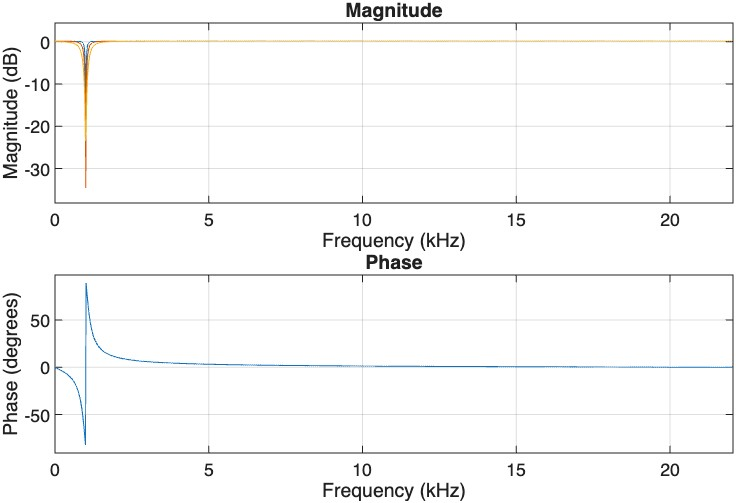
\includegraphics[width=0.48\textwidth]{image_29.jpg}\hspace{4pt}
  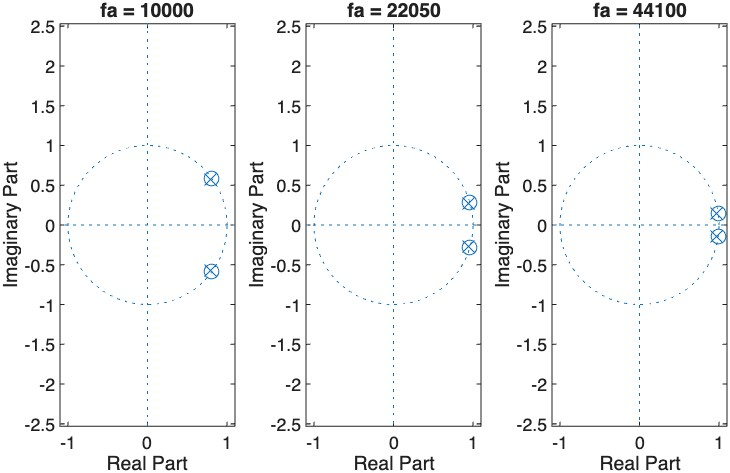
\includegraphics[width=0.48\textwidth]{image_30.jpg}
  \caption{same stop frequency, different sample rates}\label{fig:23}
\end{figure}

Used notch function to analyse magnitude, phase, pole zero plot with same stop frequency $f_s = 1000$ Hz and sample rates $f_a = 10000$, $22050$, $44100$ Hz. Higher sampling rate produces a bit wider notch in magnitude spectrum, while attenuation reaches -34 $dB$ with higher sampling rates. In pole zero plot poles and zeros together with their conjugate complex pair get closer to Re axis as $f_a$ increases. At notch frequency phase spike happens between -89 and +89 degrees because zeros on unit circle cause sign change in transfer function H(z). 

\begin{figure}[H]
  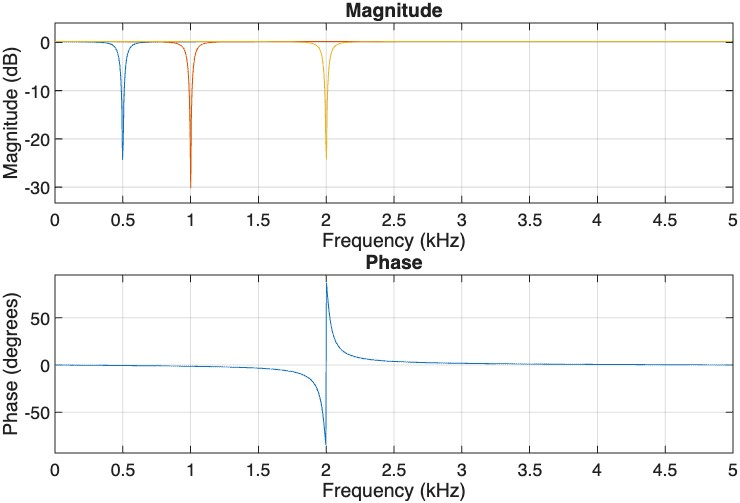
\includegraphics[width=0.48\textwidth]{image_31.jpg}\hspace{4pt}
  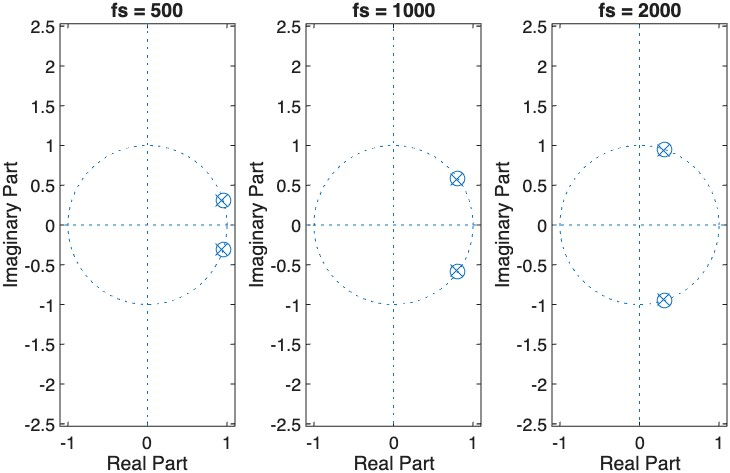
\includegraphics[width=0.48\textwidth]{image_32.jpg}
  \caption{same sample rate, different stop frequencies}\label{fig:24}
\end{figure}

Different stop frequencies $f_s = 500$, $1000$, $2000$ Hz with same sample rate $f_a = 10000$ Hz. Notch and phase shift moves to corresponding stop frequency. In pole zero plot zeros and poles get further from Re axis on unit circle as $f_s$ increases.

\codeused
\begin{matlab}
% same stop frequency, different sample rates
[b1, a1] = notchFilter(1000, 10000, 0.98);
[b2, a2] = notchFilter(1000, 22050, 0.98);
[b3, a3] = notchFilter(1000, 44100, 0.98);
freqz(b1, a1, resolution, 10000); hold on;
freqz(b2, a2, resolution, 22050); hold on;
freqz(b3, a3, resolution, 44100);

% different stop frequencies, same sample rate
[b4, a4] = notchFilter(500, 10000, 0.98);
[b5, a5] = notchFilter(1000, 10000, 0.98);
[b6, a6] = notchFilter(2000, 10000, 0.98);
freqz(b4, a4, resolution, 10000); hold on;
freqz(b5, a5, resolution, 10000); hold on;
freqz(b6, a6, resolution, 10000);
\end{matlab}

\subsubsection{(c) Analyse with your Notch filter function also the influence of the pole radius r on the characteristics of the filter with the amplitude and phase response as well plot the pole-zero maps.}

\begin{figure}[H]
  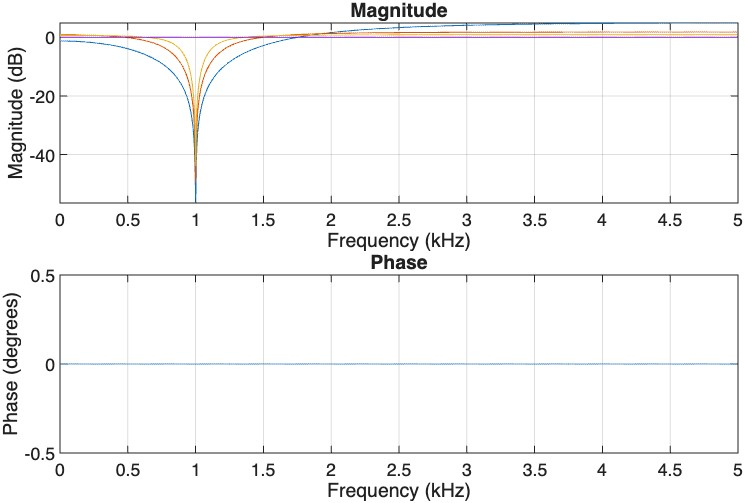
\includegraphics[width=0.48\textwidth]{image_33.jpg}\hspace{4pt}
  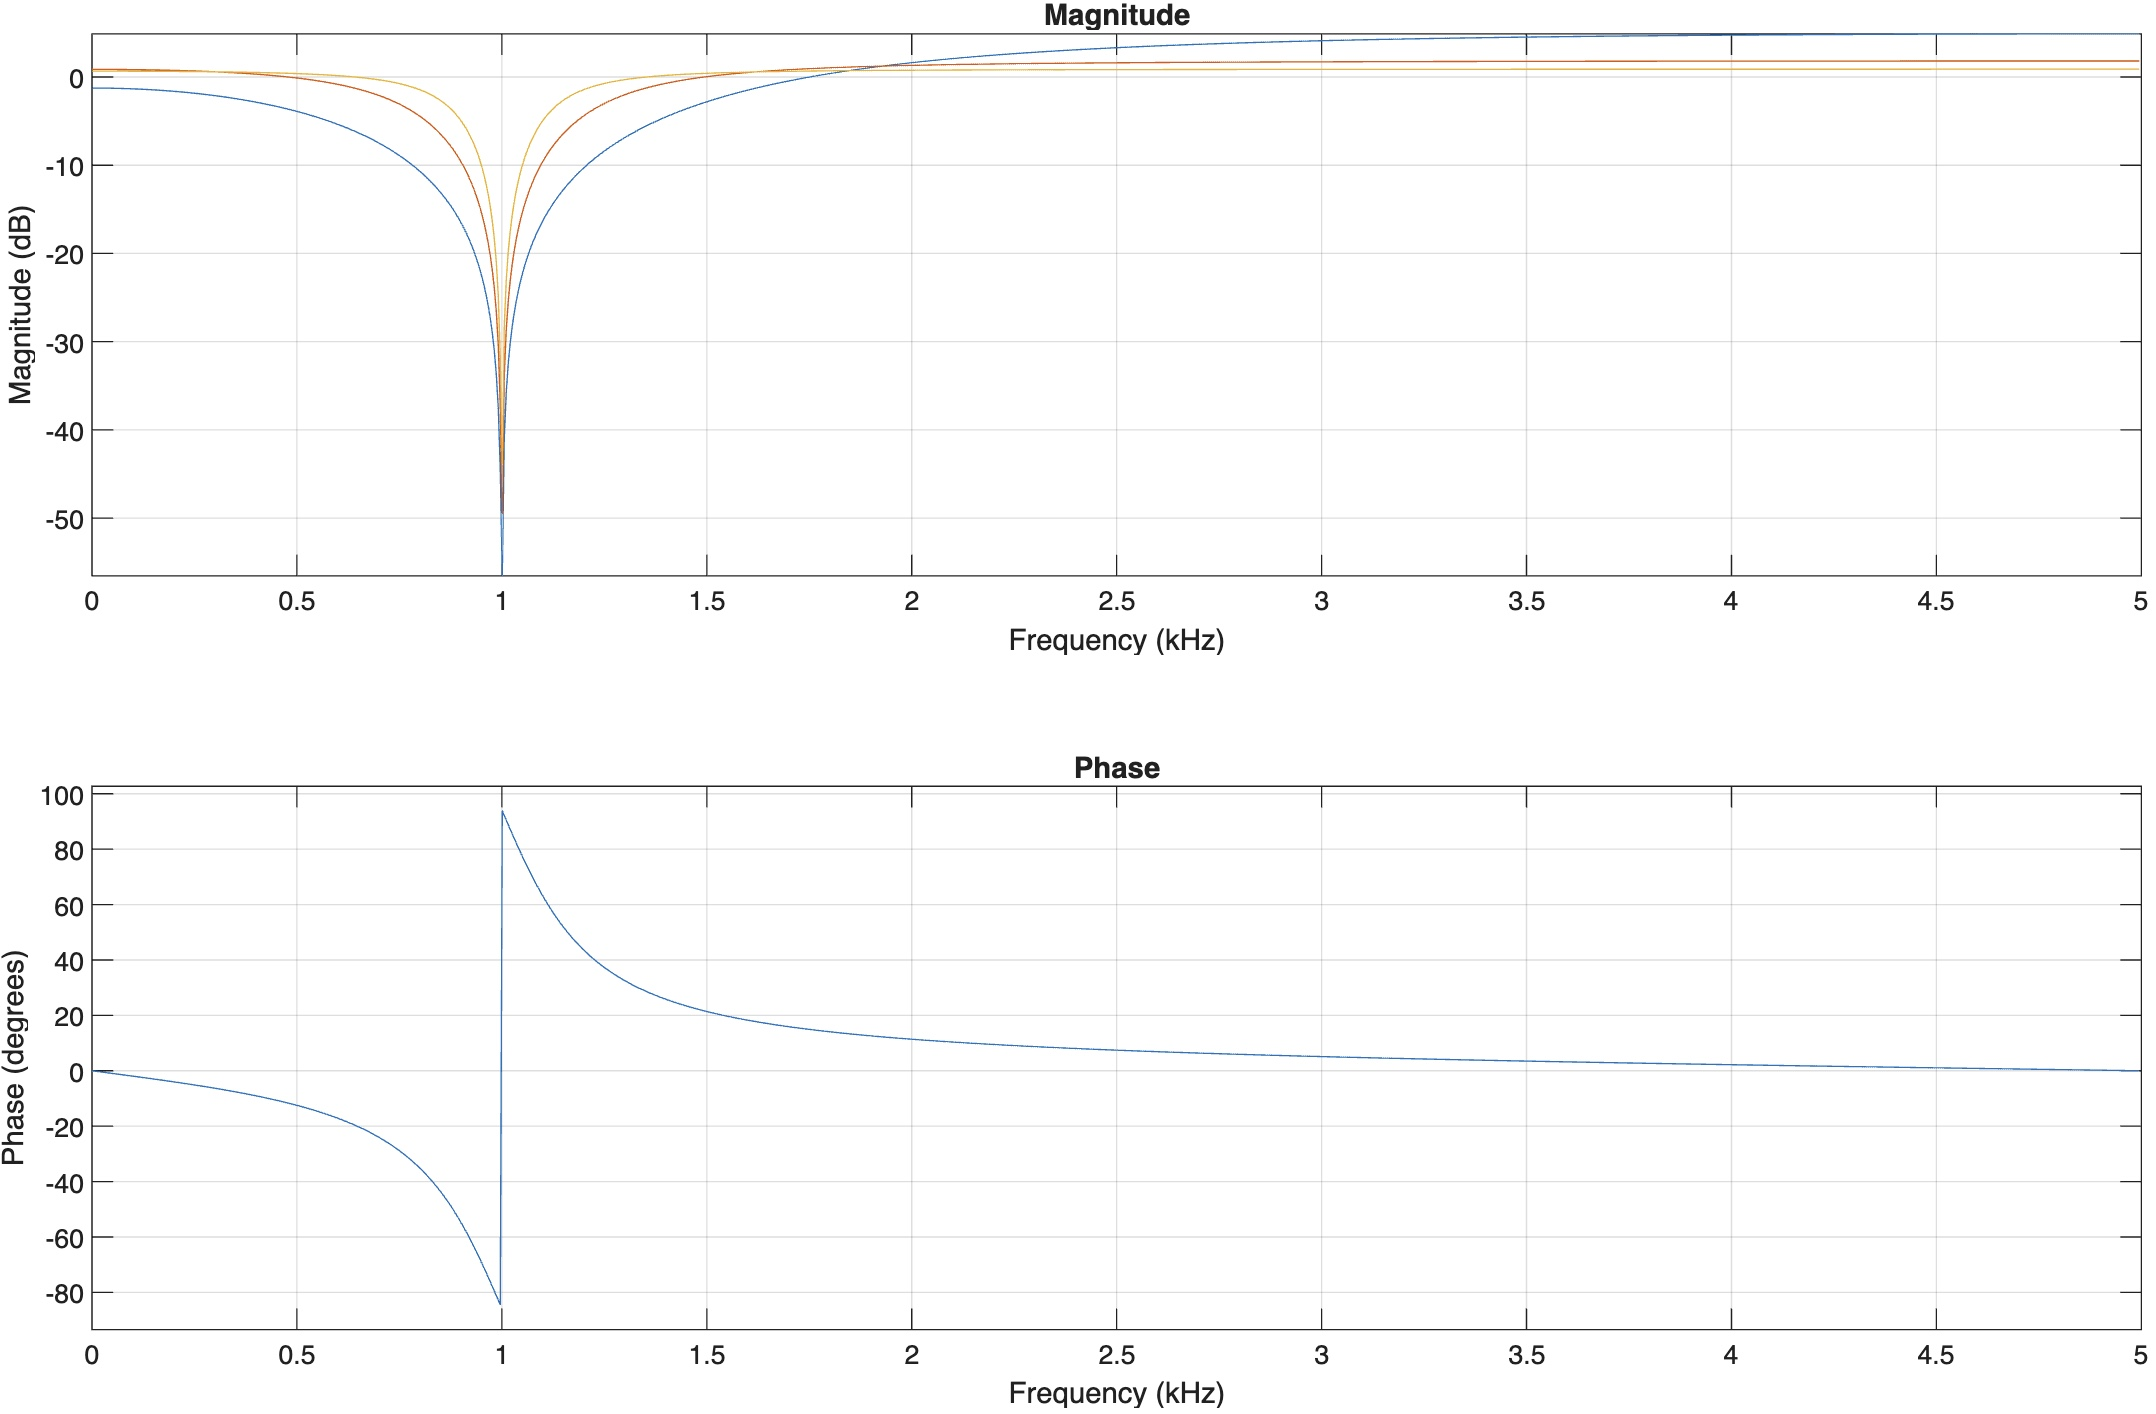
\includegraphics[width=0.48\textwidth]{image_80.png}
  \caption{influence of r on magnitude and phase}\label{fig:25}
\end{figure}

\begin{figure}[H]
  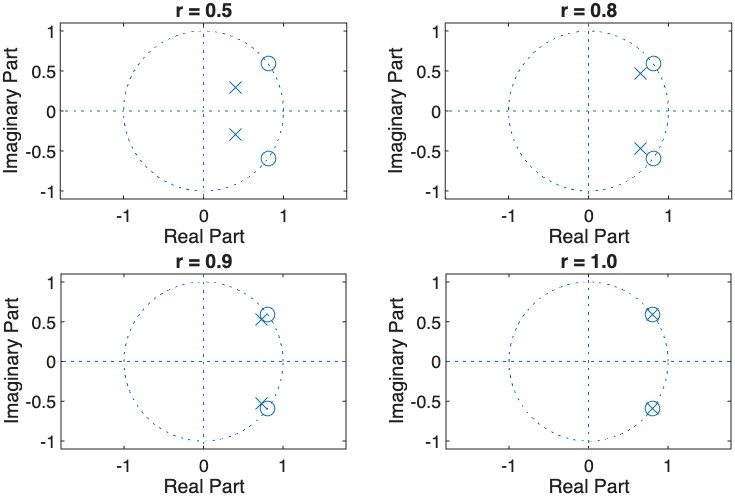
\includegraphics[width=0.6\textwidth]{image_34.jpg}
  \caption{pole zero plot for different r}\label{fig:26}
\end{figure}

Tested $r$ = 0.5, 0.8, 0.9, 1.0. Higher $r$ creates more narrow and steep notch. In pole zero plot poles move closer to unit circle as $r$ increases, expected from theoretical introduction. At $r = 1$ poles sit exactly on zeros so they cancel and $H(z) = 1$ everywhere, no filtering effect produced. Phase plot with $r = 1$ is flat at 0 degrees because numerator and denominator are identical.

\codeused
\begin{matlab}
[b7, a7] = notchFilter(1000, 10000, 0.5);
[b8, a8] = notchFilter(1000, 10000, 0.8);
[b9, a9] = notchFilter(1000, 10000, 0.9);
[b10, a10] = notchFilter(1000, 10000, 1.0);
freqz(b7, a7, resolution, 10000); hold on;
freqz(b8, a8, resolution, 10000); hold on;
freqz(b9, a9, resolution, 10000); hold on;
freqz(b10, a10, resolution, 10000);
\end{matlab}

\subsubsection{(d) Correct the gain factor for your notch filter function.}

Without correction passband gain is only largely constant but not exactly 1. Gain correction scales $b$ coefficients so that $H(z = 1) = 1$. Factor $b_0 = |{\sum a}| / |{\sum b}|$ is ratio of denominator to numerator evaluated at $z = 1$ which is DC component at 0 Hz.

\codeused
\begin{matlab}
function [b, a] = notchFilterGC(fs, fa, r)
    w0 = 2 * pi * fs / fa;
    b = [1, -2 * cos(w0), 1];
    a = [1, -2 * r * cos(w0), r^2];
    % make H(z = 1) = 1
    b0 = abs(sum(a)) / abs(sum(b));
    b = b0 * b;
end
\end{matlab}

\subsection{Laboratory 2 -- Design a Comb filter out of a Butterworth low-pass filter with 3 repetitions}

Comb filters are used to remove interference with harmonics at multiples of fundamental frequency that can be achieved by using notch filter as comb filter.

Constructed by inserting zeros between original filter coefficients which increases sampling frequency while keeping the original filter shape unchanged. Each inserted zero extends frequency range by original $\omega_s/2$, so inserting $n$ zeros produces ($n+1$) copies of filter shape. Thus, inserting $n$ zeros replaces $z^{-1}$ with $z^{-(n+1)}$ in the transfer function. 

\begin{equation}
  G(z) = b_0 + b_1 z^{-1} + b_2 z^{-2}
  \;\;\Rightarrow\;\;
  G(z) = b_0 + b_1 z^{-(n+1)} + b_2 z^{-2(n+1)}
  \tag{3}
\end{equation}

Sampling frequency stays the same but original notch filter shape gets compressed and repeated $n+1$ times between 0 and $\omega_s/2$.

For IIR comb filter zeros must be inserted between both $b_n$ and $a_n$ coefficients.

\begin{figure}[H]
  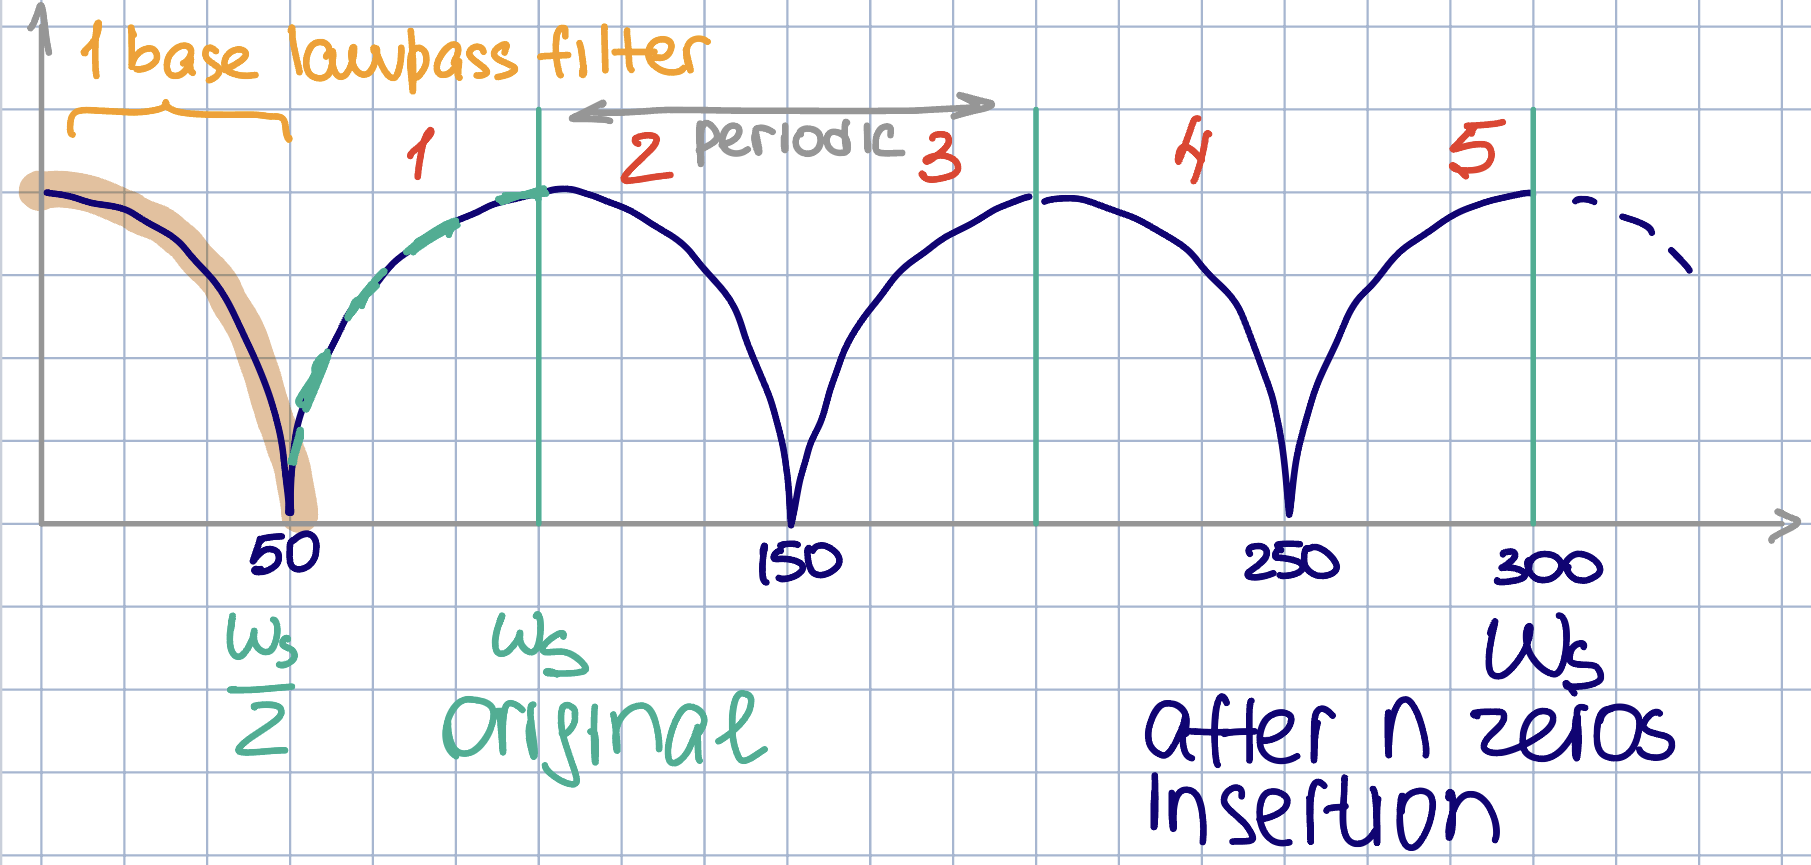
\includegraphics[width=0.48\textwidth]{image_81.png}\hspace{4pt}
  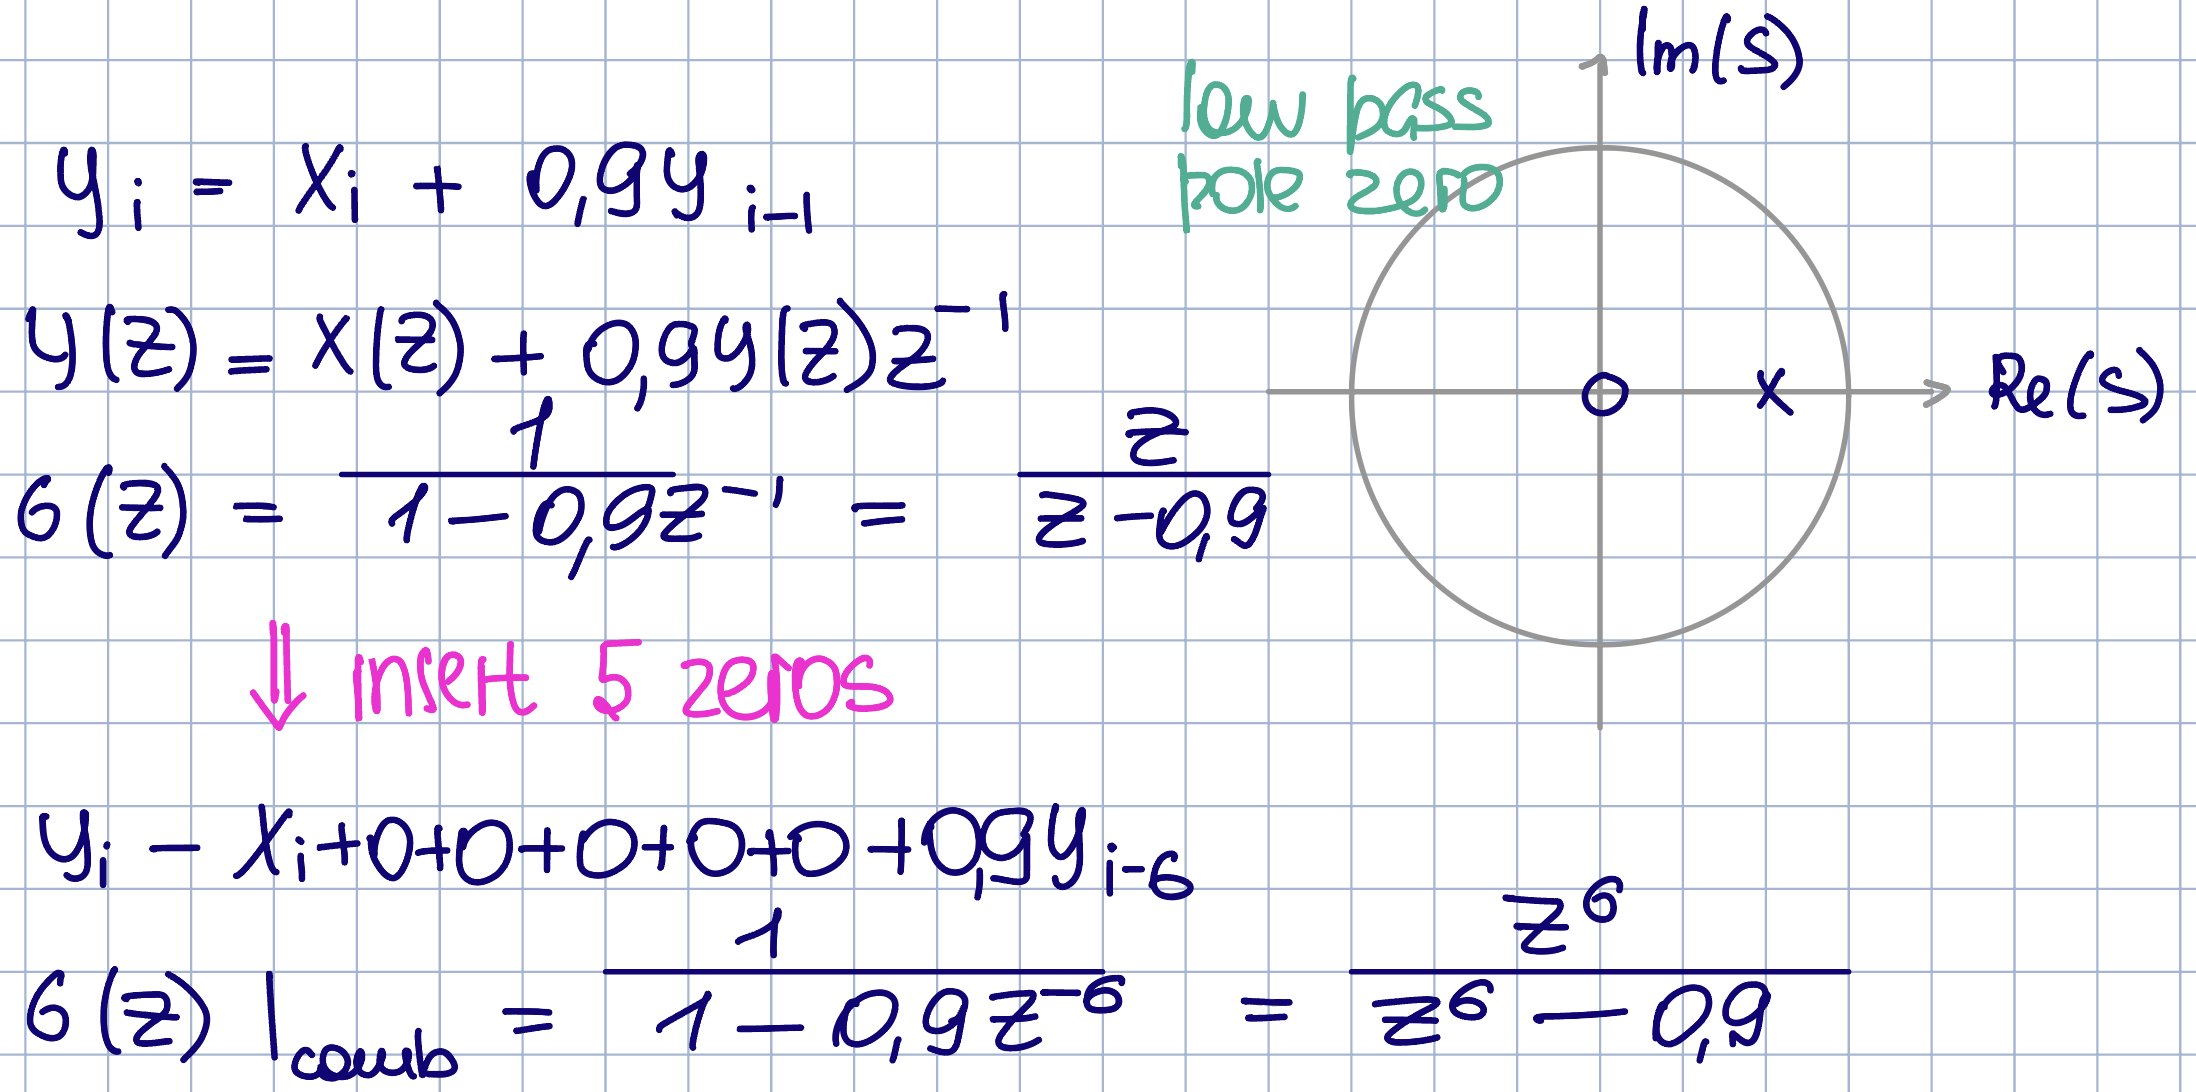
\includegraphics[width=0.48\textwidth]{image_82.png}
  \caption{comb filter zero insertion principle based on lowpass example}\label{fig:27}
\end{figure}

\subsubsection{(a) Write a Comb filter function which can design a Comb filter by taking the following parameters:}

% given on the exercise sheet:
\begin{itemize}
  \item filter coefficients b; filter coefficients a; repetitions n
\end{itemize}

\begin{figure}[H]
  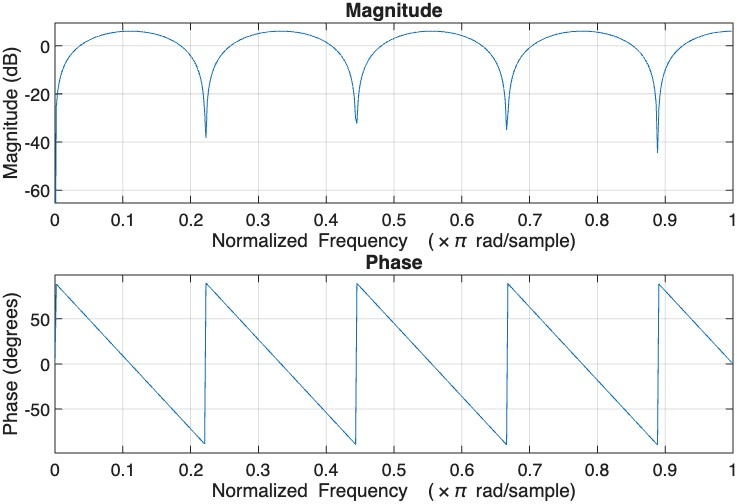
\includegraphics[width=0.48\textwidth]{image_35.jpg}\hspace{4pt}
  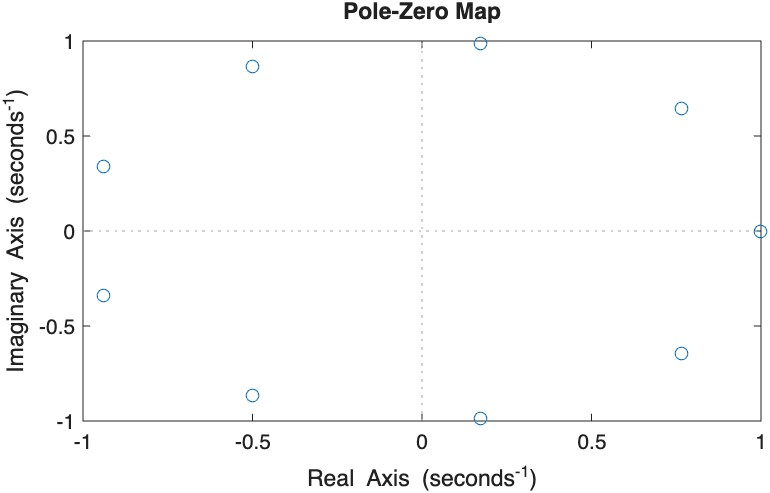
\includegraphics[width=0.48\textwidth]{image_36.jpg}
  \caption{basic comb filter frequency response and pole-zero map}\label{fig:28}
\end{figure}

Basic comb filter with $r$ = 0.9999995 and $L_f$ = 9 uses FIR structure with $a = 1$ so only zeros, no poles. 9 zeros are placed near unit circle creating equally spaced notches across 0 to $\pi$.

\codeused
\begin{matlab}
r = 0.9999995; Lf = 9;
b = [1 zeros(1, Lf - 1) -r^Lf]; a = 1;
freqz(b, a); pzmap(tf(b, a));
function [b_comb, a_comb] = combFilter(b, a, n)
    b_comb = zeros(1, (length(b) - 1) * n + 1);
    a_comb = zeros(1, (length(a) - 1) * n + 1);
    % original coefficients every n th position
    b_comb(1:n:end) = b;
    a_comb(1:n:end) = a;
end
\end{matlab}

\subsubsection{(b) Use your Comb filter function and analyse it with the amplitude and phase response of the filter.}

\begin{figure}[H]
  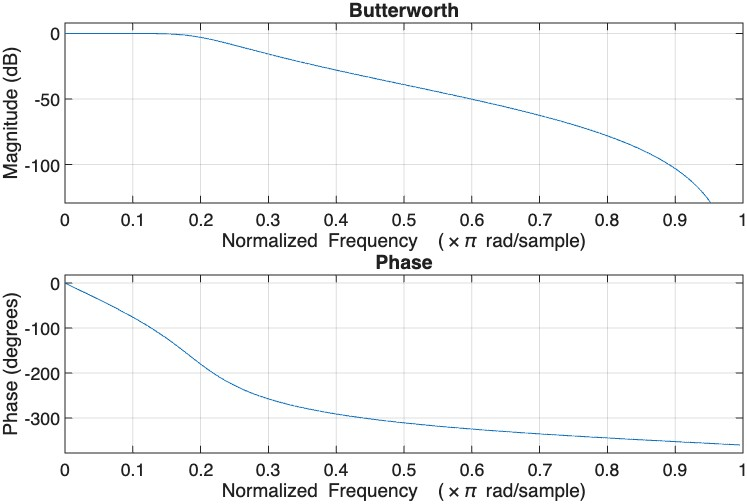
\includegraphics[width=0.32\textwidth]{image_37.jpg}\hspace{4pt}
  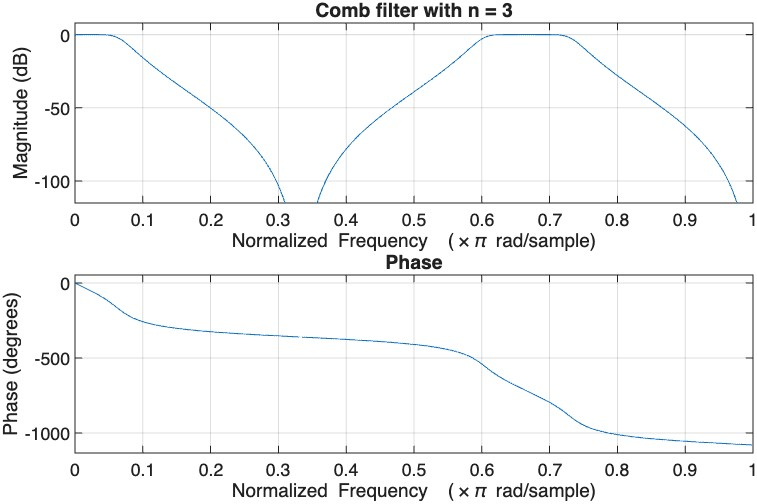
\includegraphics[width=0.32\textwidth]{image_38.jpg}\hspace{4pt}
  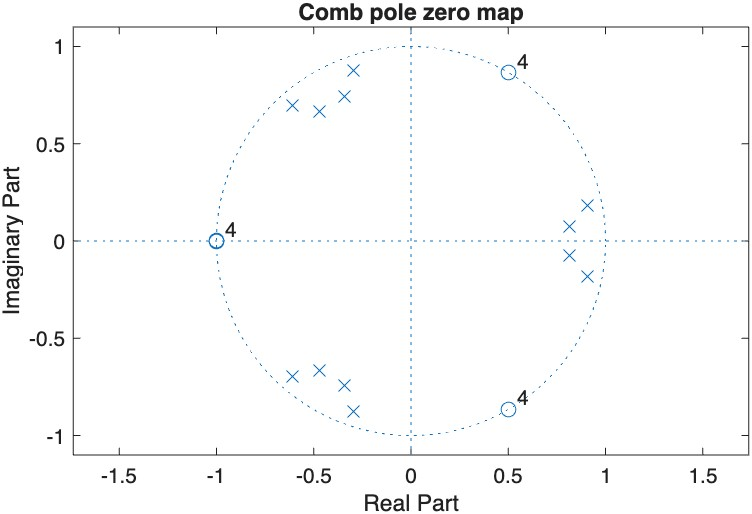
\includegraphics[width=0.32\textwidth]{image_39.jpg}
  \caption{butterworth lowpass, comb filter with n=3, and pole-zero map}\label{fig:29}
\end{figure}

Used order $N$ = 4 Butterworth lowpass with cutoff at $0.2\pi$, meaning that transfer function has 4 poles and 4 zeros. combFilter with $n = 3$ inserts 3 zeros between each coefficient. Lowpass filter shape is repeated 3 times across 0 to $\pi$, thus phase also repeats 3 times being compressed to $0.33\pi$ which is $1/3$ of original lowpass filter range between 0 and $\pi$. Poles and zeros are copied 3 times at multiples of $0.33\pi$ frequency.

\codeused
\begin{matlab}
[b_lp, a_lp] = butter(4, 0.2);
% comb with 3 repetitions
[b_comb, a_comb] = combFilter(b_lp, a_lp, 3);
freqz(b_lp, a_lp, 1024); freqz(b_comb, a_comb, 1024);
zplane(b_comb, a_comb);
\end{matlab}

\subsection{Homework 2 (Implement your own Notch-Comb filter function)}

\subsubsection{Implement your own Notch-Comb filter function with the following parameters:}

% given on the exercise sheet:
\begin{itemize}
  \item sample rate fa; repetitions n; pole radius r
\end{itemize}
Show the results with appropriate diagrams

\begin{figure}[H]
  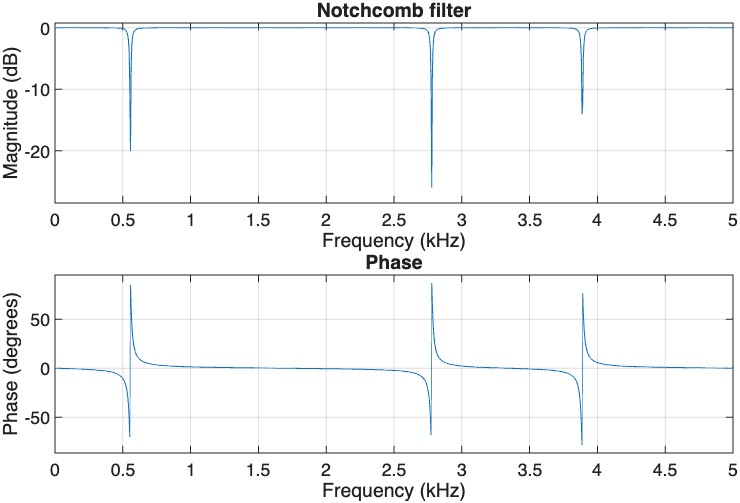
\includegraphics[width=0.48\textwidth]{image_40.jpg}\hspace{4pt}
  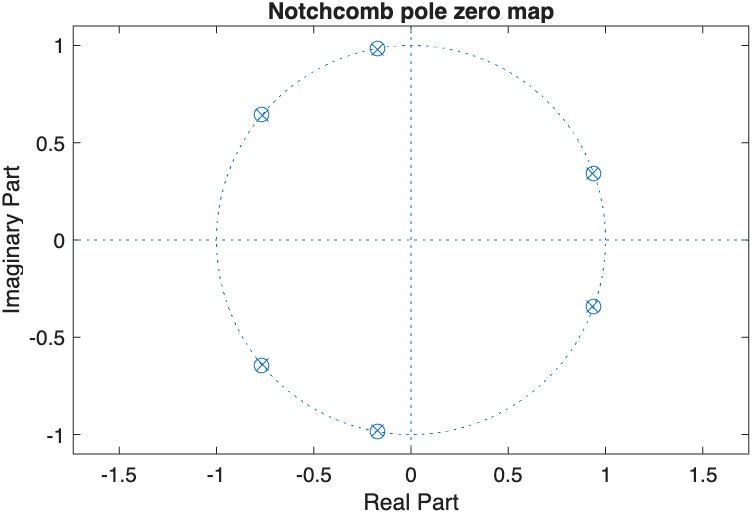
\includegraphics[width=0.48\textwidth]{image_41.jpg}
  \caption{notch-comb filter frequency response and pole-zero map}\label{fig:30}
\end{figure}

For $f_a = 10000$ Hz, $n = 3$, $r = 0.98$ notches are at 556, 2778, 3889 Hz, 3 notches produced, poles are close to zeros, thus notches are very steep and narrow. Gain correction keeps passband flat at 0 dB between notches.

\begin{figure}[H]
  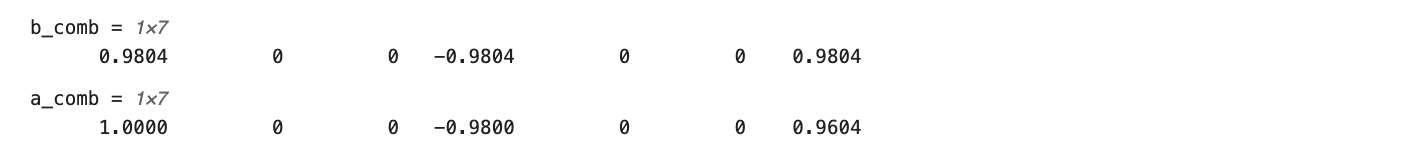
\includegraphics[width=0.6\textwidth]{image_42.jpg}
  \caption{notch-comb filter coefficients}\label{fig:31}
\end{figure}

Only 7 coefficients needed compared to FIR.

\codeused
\begin{matlab}
function [b_comb, a_comb] = notchCombFilter(fa, n, r)
    % notch at fa/2 divided by n repetitions
    fs = fa / (2 * n);
    % gain corrected notch
    [b, a] = notchFilterGC(fs, fa, r);
    % repeat n times with z -> z^n
    [b_comb, a_comb] = combFilter(b, a, n);
end
fa = 10000; n = 3; r = 0.98;
[b_notchcomb, a_notchcomb] = notchCombFilter(fa, n, r);
freqz(b_notchcomb, a_notchcomb, 1024, fa);
zplane(b_notchcomb, a_notchcomb);
\end{matlab}

\clearpage
\section{Lab exercise 3: Adaptive Filter Design}

Main idea of adaptive filtering is to dynamically adjust filter transfer function based on the noise coming to the listener that is constanly changing in real time with signal (Figure~\ref{fig:301}). It is impossible to know noise trasnfer function in advance, it can differ. To remove noise coming mixed with true signal, noise signal must be added with a minus sign and adaptive filter transfer function must be always changed so that it cancels out real noise distortion transfer function. This way system can get as close as possible to transfer function of incoming noise and cancel it.

\begin{figure}[H]
  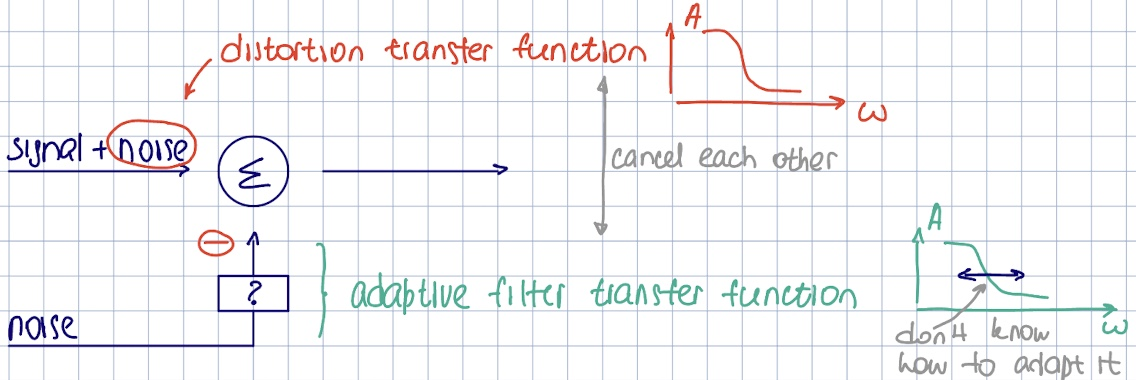
\includegraphics[width=0.6\textwidth]{image_85.png}
  \caption{main idea of adaptive filter}\label{fig:301}
\end{figure}

To adjust filter transfer function dynamically, real time resulting signal measure and error term must be introduced, to give meaningful direction to adapt. Since noise is mostly random, it has high power $P$. Therefore, power of output signal $y$ coming out of the system must be measured, assuming that noise is stationary, equivalently constant in freqeuncy and amplitude. Adaptive filter aims to have noise interference signal $a_i$ and modelled noise by adaptive filter $b_i$ to be equal, then meaningful error is error signal $e$, which is the difference between real signal $s_i$ = $x_i$ and output signal $y_i$ resulting from the adaptive filter (Figure~\ref{fig:302}). Error term equation is $e_i$ = $x_i$ - $y_i$.

If there is no noise interference, then error term would be zero, and trivially its power $P_e$ would also be zero. If noise is present and strong, error term would be large, and its power $P_e$ would emphasize it even more because of squaring the difference term.

\begin{figure}[H]
  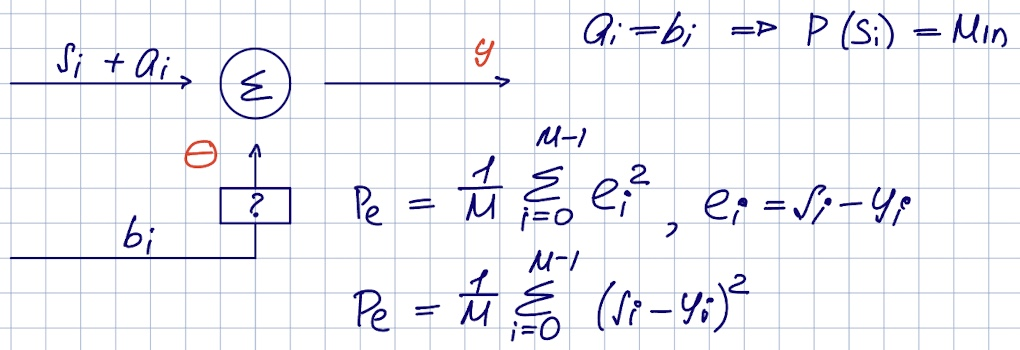
\includegraphics[width=0.6\textwidth]{image_86.png}
  \caption{error term in adaptive filter}\label{fig:302}
\end{figure}

Output signal $y$ can be filtered using simple FIR second order filter, which is same as convolution of filter coefficients $b_0$, $b_1$, $b_2$ with input signal samples. FIR is only safe option, because adjusting IIR feedback coefficients can put poles outside of unit circle in z-plane and make system unstable. Thus, what is left is to plug in $y$ FIR filtering formula into error term power equation $P_e$ and form relation of one of the coefficients and $P_e(b_i)$ expressed as parabola.

After inserting $y_i = b_0 * x_i + b_1 * x_{i-1} + b_2 * x_{i-2}$ FIR filtered formula into $P_e$ and grouping terms that depend on $b_1$ separately from terms that do not depend on it into $A_i = s_i - b_0 * x_i - b_2 * x_{i-2}$ coefficient, $P_e(b_1)$ becomes parabola with minimum at optimal, equivalently minimum value of FIR filter coefficient $b_1$ (Figure~\ref{fig:303}). Same mechanism applies for all FIR coefficients $b_n$. 

\begin{figure}[H]
  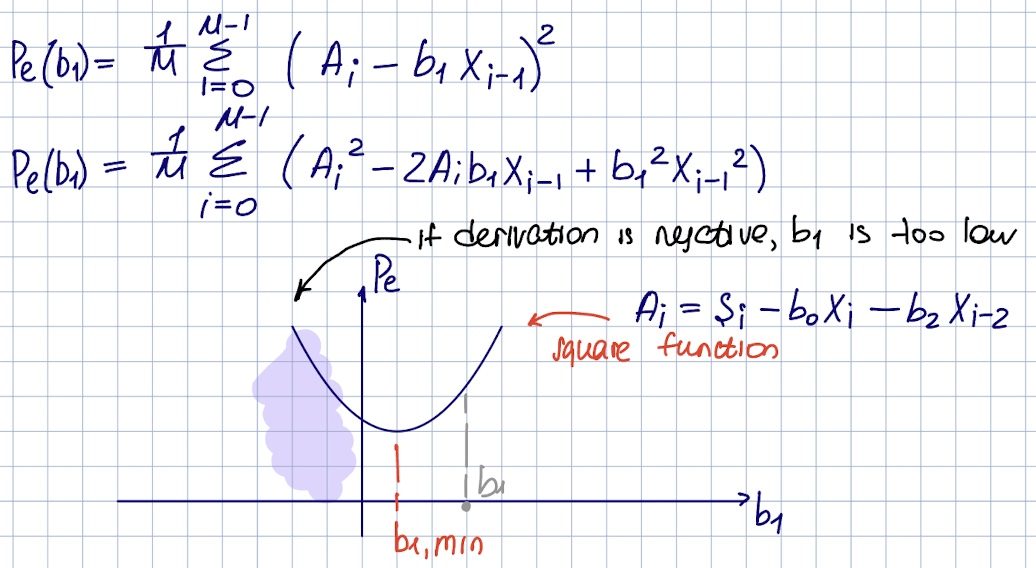
\includegraphics[width=0.6\textwidth]{image_88.png}
  \caption{error term in adaptive filter}\label{fig:303}
\end{figure}

Quadratic gives desired useful gradient of improvement since derivative at any value of $b_n$ indicates the direction and magnitude of error term minimization needed (Figure~\ref{fig:304}). If derivative is positive, $b_n$ is too high and must be reduced. If negative, $b_n$ must be increased. 

\begin{figure}[H]
  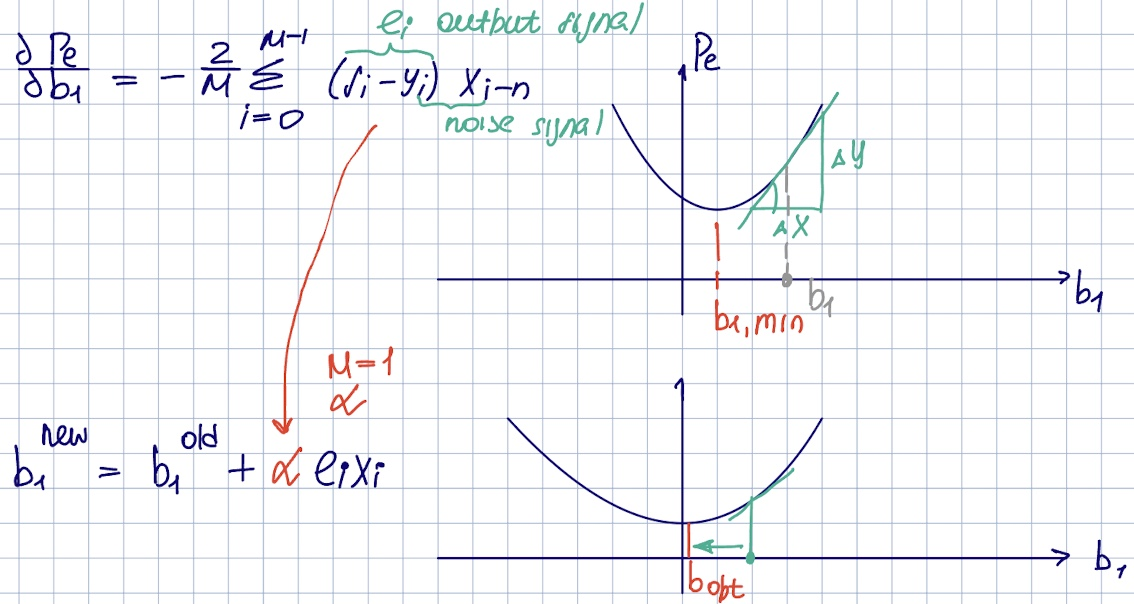
\includegraphics[width=0.6\textwidth]{image_87.png}
  \caption{error term gradient}\label{fig:304}
\end{figure}

With $M = 1$, coefficients are updated after every single sample instead of averaging gradient over a block of $M$ samples. Factor of 2 comes from derivative of squared error term $(s_i - y_i)^2$, minus sign from gradient and minus from gradient descent direction cancel out. 

FIR filter coefficients are updated with learning rate (adaptation coefficient) $\mu$ or $\alpha$ on sketch I made (Figure~\ref{fig:304}). Smaller $\mu$ gives more accurate result but converges towards optimum slower. Larger $\mu$ leads to faster adaptation but can overshoot optimum. Resulting least mean squared update rule for each coefficient after every sample, I later use to complete given template for adaptive filtering, is (Equation~\ref{eq:lms}).

\begin{equation}
b_n^{new} = b_n^{old} + 2 * \mu * e_i * x_{i-n}
\label{eq:lms}
\end{equation}

So basic idea of adapting modelled noise tranfer function to cancel out noise is updating FIR filtered signal coefficients based on gradient of error term power with respect to corresponding filter coefficient. This approach is effective, but also should be noted that adjusting one coefficient $b_1$ influences others, thus optimal $b_1$ does not guarantee optimal $b_0$ and $b_2$. If $b_1$ reached optimum, and later $b_0$ is adjusted, $b_1$ can be no longer optimum.

\subsection{Laboratory 3 -- Use the Adapt\_Filter\_Template.m and complete the code of the adaptive filter routine.}

Diagram given shows that degraded signal $d(k)$ contains useful signal mixed with noise. Noise source provides reference signal $x(k)$, which adaptive FIR filter processes into modelled noise $y(k)$. Error signal $e(k) = d(k) - y(k)$ is the recovered signal and at the same time feedback to the adaptive filter. Filter coefficients $b_n$ are updated after each sample using FIR coefficients update rule (Figure~\ref{fig:304}), where gradient of error power $P_e$ with respect to $b_n$ converges each coefficient towards its optimum on the parabola (Figure~\ref{fig:303}).

% diagram given
\begin{figure}[H]
  \centering
  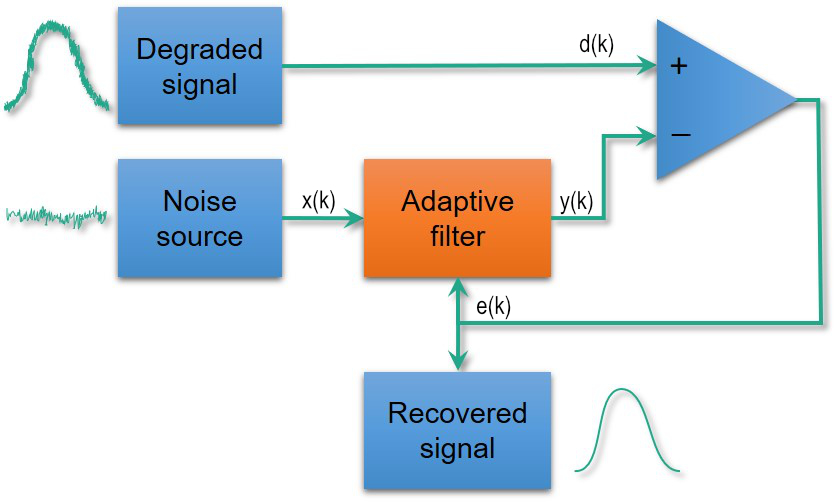
\includegraphics[width=0.6\textwidth]{image_43.png}\par
  \vspace{4pt}
  {\textbf{Fig. 1:} LMS - Adaptive Filter Concept}
\end{figure}

Template given \hyperlink{code:templateSignals}{generate signal} with undisturbed sinusoid $s_0$ at 50 Hz and noise interference as Gaussian noise filtered through FIR order 10 as interference $x$. Interference is added to undisturbed sinusoid signal through transfer function $[0.2, 0.5, 0.8, 0.5, 0.2]$ to form degraded signal $d(k)$. Adaptive FIR filter of order $N = 4$ with adaptation parameter $\mu$ is initialized with zero coefficients. 

Template gives outer sample loop and inner coefficient loops. Thus, only lms update rule using final equation (\ref{eq:lms}) from theoretical introduction for $b$ coefficients needs to be implemented. One more thing missing is $mu$ learning rate.

\codeused
\hypertarget{code:templateSignals}{}
\begin{matlab}
% Settings
N = 4;
% Filter Order
dt = 1e-4;
% Sample Time
tend = 5;
% Signal length
t = 0:dt:tend-dt;
% Undisturbed Signal
s0 = sin(2*pi*50*t);
% Interference
xx = 0.5*randn(size(t));
b = fir1(10, 0.8);
x = filter(b, 1, xx);
% Part of the Interference added to the undisturbed Signal
sn = filter([0.2 0.5 0.8 0.5 0.2], 1, x);
% Disturbed Signal
d = s0 + sn;
% adaptation parameter mu - MISSING!
mu = ....; % find a good adaptation parameter mu
% Adaptive Filter
b = zeros(N+1,1); % Initialising Coefficients
e = zeros(size(x)); % Filtered Signal as difference (d-y)
bb = zeros(N+1,length(x)-N+1);  % to record new b-Coefficients
% Adaptive Filter routine (with recorded adapted b coefficients)
    for i=N+1:1:length(x)
        y = 0;  
        for n=1:1:N+1
            % Output from Filtering
        end
        % Calculate filtered Signal as difference (d-y)
		for n=1:1:N+1
        % Calculate new b coefficients - MISSING!
        end
        % Record old b coefficients
    end
\end{matlab}

To check how filtering works I ran script and plotted time domains of undisturbed signal, interference signal, disturbed signal, and resulting filtered signal. Found optimal $mu$ learning rate by trying different values 0.01, 0.001, 0.0001, and checking how close is filtered signal to its undisturbed time domain plot visually.

\begin{figure}[H]
  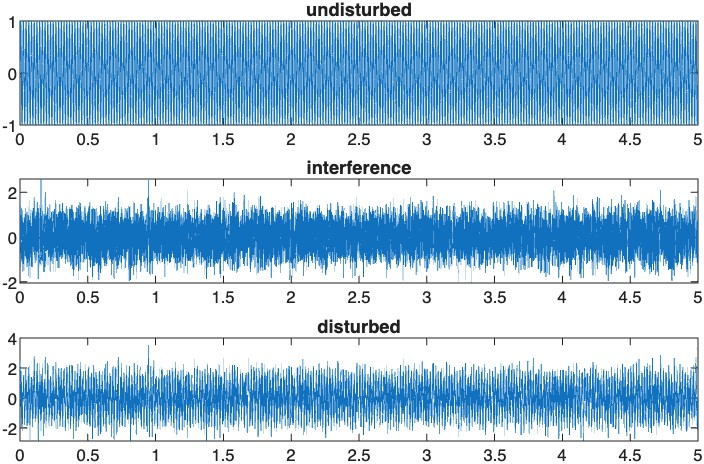
\includegraphics[width=0.48\textwidth]{image_44.jpg}\hspace{4pt}
  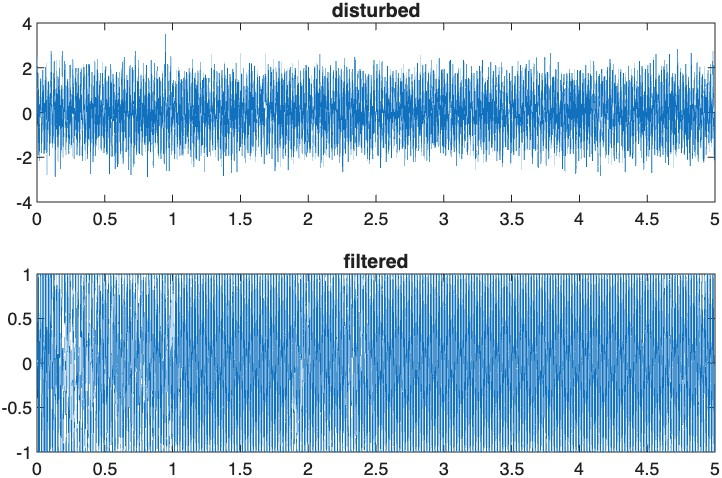
\includegraphics[width=0.48\textwidth]{image_45.jpg}
  \caption{input signals and filtered result}\label{fig:32}
\end{figure}

Based on output in Figure~\ref{fig:32}, it can be seen that adaptive FIR filtering works well and time domain plots of filtered and undisturbed signals are mostly same, except some delay of FIR filter to be able to work, which took about 1 second, until filtering became almost perfect.

\begin{figure}[H]
  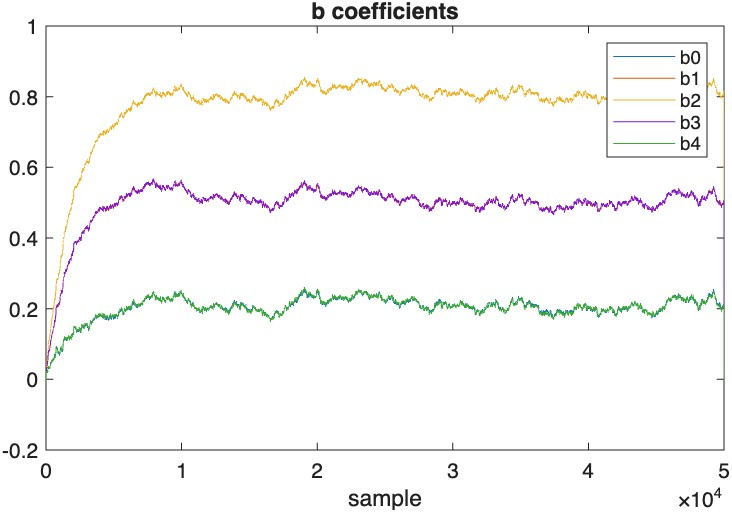
\includegraphics[width=0.48\textwidth]{image_46.jpg}\hspace{4pt}
  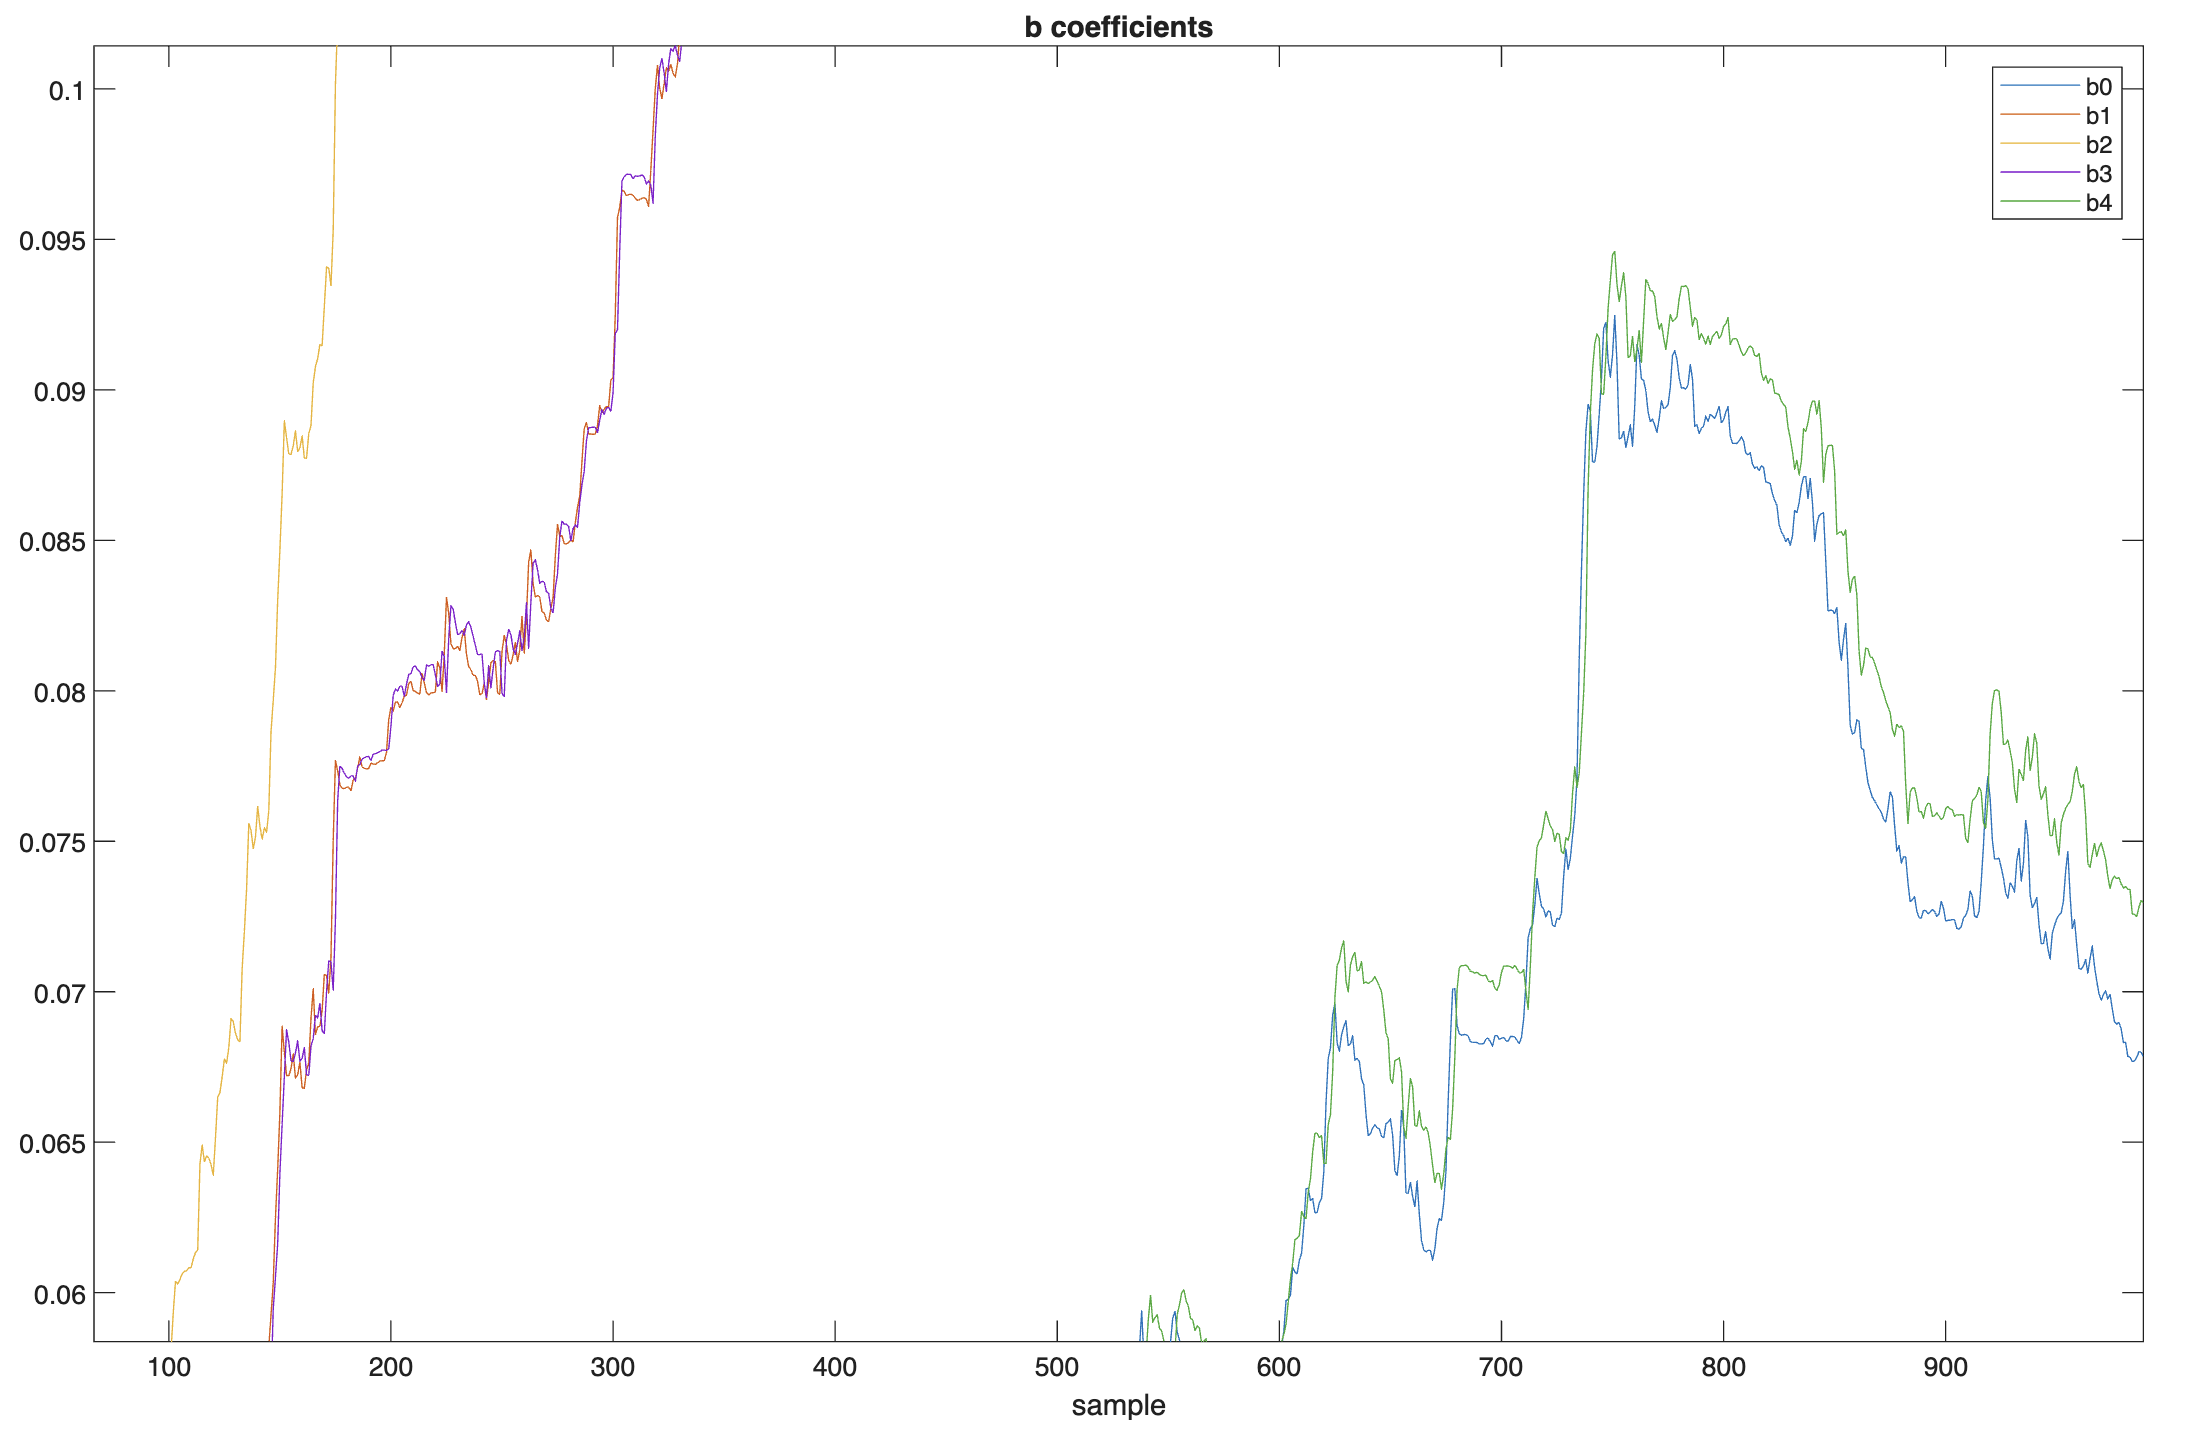
\includegraphics[width=0.48\textwidth]{image_99.png}
  \caption{b coefficient convergence}\label{fig:33}
\end{figure}

FIR filter coefficients $b_0$ = $b_4$, $b_1$ = $b_3$, $b_2$ are contributing equally in filtering converging to respective values of 0.2, 0.5, 0.8 after about 1 second (Figure~\ref{fig:33}), almost exactly with some variance matching interference transfer function coefficients $[0.2, 0.5, 0.8, 0.5, 0.2]$ from the \hyperlink{code:templateSignals}{template}.

\codeused
\begin{matlab}
% Plot disturbed and filtered Signal
figure; subplot(2,1,1); .. title('disturbed'); subplot(2,1,2); .. title('filtered');
% Plot recorded b coefficients in time
figure; plot(bb'); ... legend('b0','b1','b2','b3','b4');
\end{matlab}

\subsubsection{(a) Check your adaptive filter routine if it is reconstructing the original signal.}

\begin{figure}[H]
  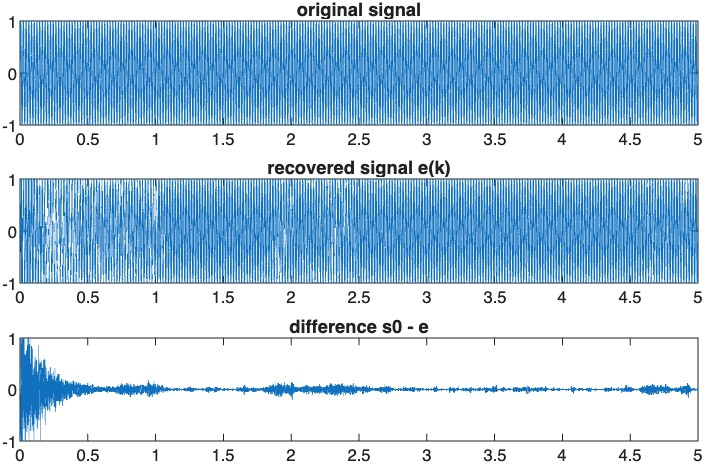
\includegraphics[width=0.6\textwidth]{image_47.jpg}
  \caption{original vs recovered signal and difference}\label{fig:34}
\end{figure}

TODO

\subsubsection{(b) Use different \texorpdfstring{$\mu$}{µ} and validate their performance via the b coefficients accordingly to the adaptation in time.}

\begin{figure}[H]
  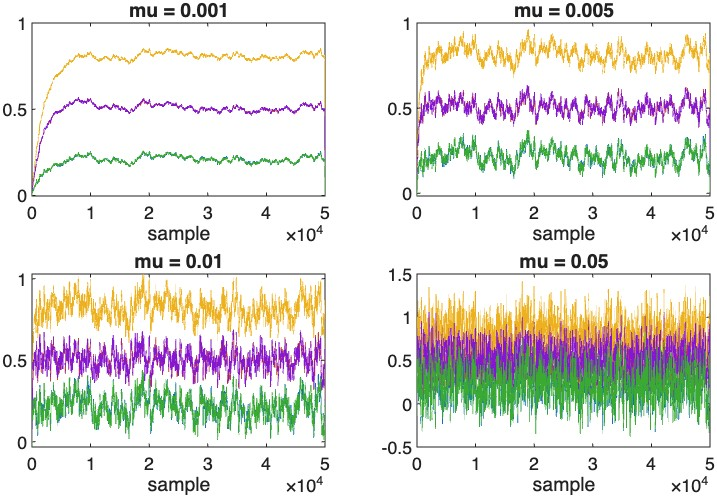
\includegraphics[width=0.6\textwidth]{image_48.jpg}
  \caption{b coefficient convergence for different mu values}\label{fig:35}
\end{figure}

TODO

\subsection{Laboratory 3 -- Adapt your filter routine to be able to read any Wave-Soundfile where in Channel\_1 the samples of the disturbed signal and Channel\_2 the samples of the interference (noise signal) is stored.}

\subsubsection{(a) Test your filter routine with the given Soundfile sound.wav}

\begin{figure}[H]
  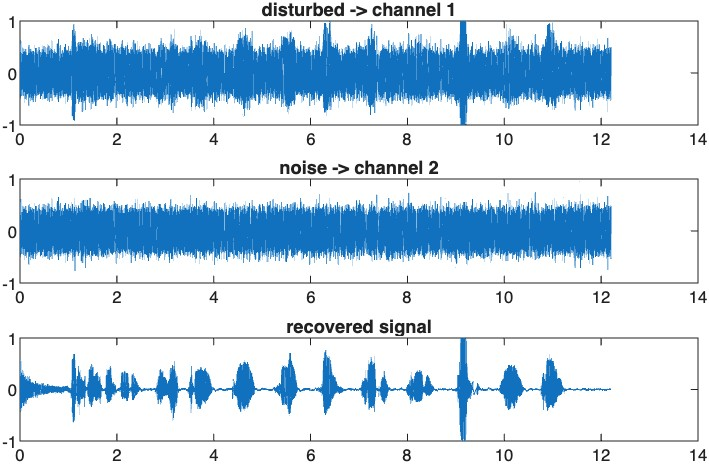
\includegraphics[width=0.6\textwidth]{image_49.jpg}
  \caption{sound.wav adaptive filtering}\label{fig:36}
\end{figure}

\begin{figure}[H]
  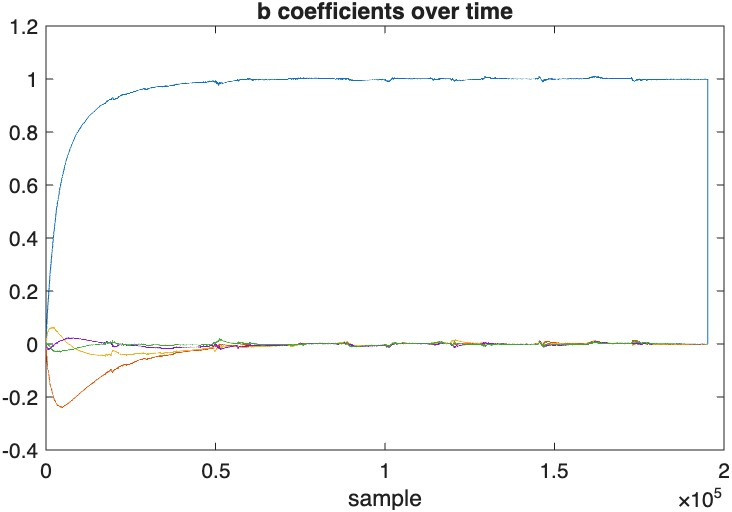
\includegraphics[width=0.6\textwidth]{image_50.jpg}
  \caption{sound.wav b coefficients over time}\label{fig:37}
\end{figure}

TODO

% =====================================================================
%  LAB 4 -- 2D-Filter and Image Processing
%  Headings copied word for word from DSP2_Lab4_Exercise.pdf
% =====================================================================
\clearpage
\section{Lab exercise 4: 2D-Filter and Image Processing}

TODO: chapter introduction -- theory about histogram equalisation,
gamma correction and image filtering.

\subsection{Laboratory 4 -- Perform the following procedure of a automatic histogram equalisation:}

\subsubsection{(a) build a histogram of the pixel values}

\begin{figure}[H]
  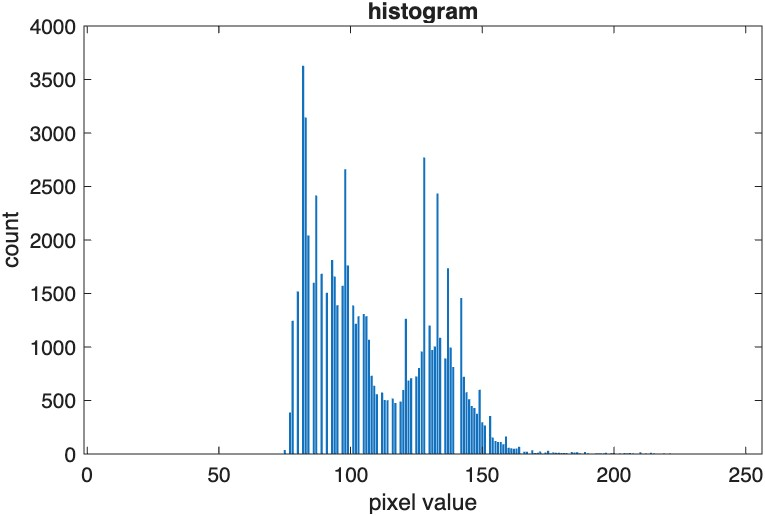
\includegraphics[width=0.6\textwidth]{lab4-histogram.jpg}
  \caption{histogram of pout.gif pixel values}\label{fig:l4-histogram}
\end{figure}

TODO

\subsubsection{(b) build the cumulative sum of this histogram}

\begin{figure}[H]
  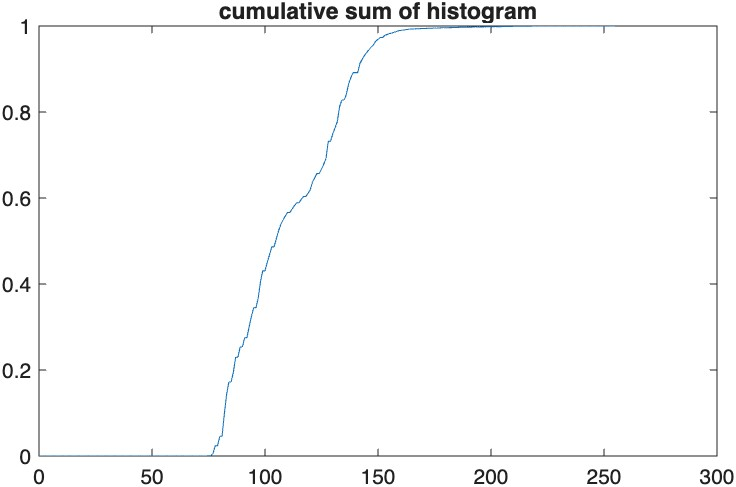
\includegraphics[width=0.6\textwidth]{lab4-cumulative.jpg}
  \caption{cumulative sum of histogram}\label{fig:l4-cumulative}
\end{figure}

TODO

\subsubsection{(c) normalise this cumulative sum to the max. pixel value}

TODO

\subsubsection{(d) use this as a mapping from old-new pixel values (lookup-table)}

TODO

\subsubsection{(e) Test your algorithm on pout.gif show the original picture as well both histograms and the resulting picture.}

\begin{figure}[H]
  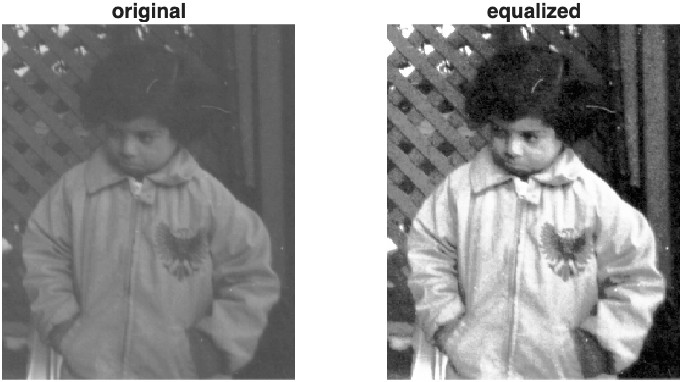
\includegraphics[width=0.48\textwidth]{lab4-equalized.jpg}\hspace{4pt}
  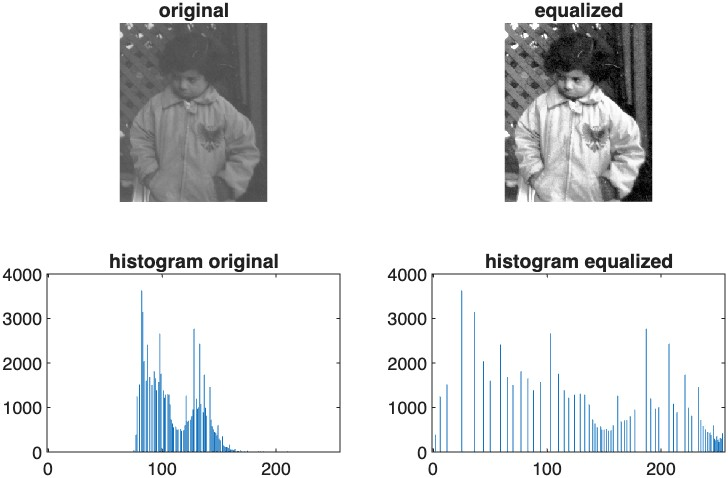
\includegraphics[width=0.48\textwidth]{lab4-equalized-comparison.jpg}
  \caption{equalized image and histogram comparison}\label{fig:l4-equalized}
\end{figure}

TODO

\subsubsection{(f) Make a comparison to the histeq function of matlab.}

\begin{figure}[H]
  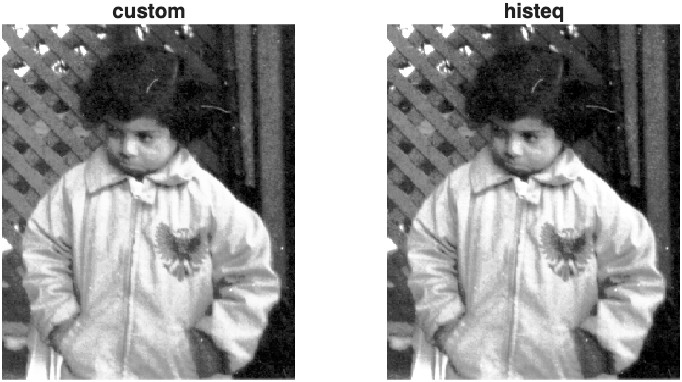
\includegraphics[width=0.6\textwidth]{lab4-histeq-comparison.jpg}
  \caption{custom equalization vs matlab histeq}\label{fig:l4-histeq}
\end{figure}

TODO

\subsection{Laboratory 4 -- Built your own gamma-correction function by using the template gctemp.m:}

\subsubsection{(a) Test the template with different gammas}

\begin{figure}[H]
  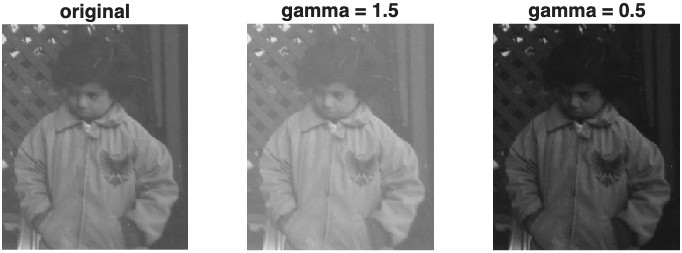
\includegraphics[width=0.6\textwidth]{lab4-gamma-pout.jpg}
  \caption{gamma correction on pout.gif}\label{fig:l4-gamma-pout}
\end{figure}

\begin{figure}[H]
  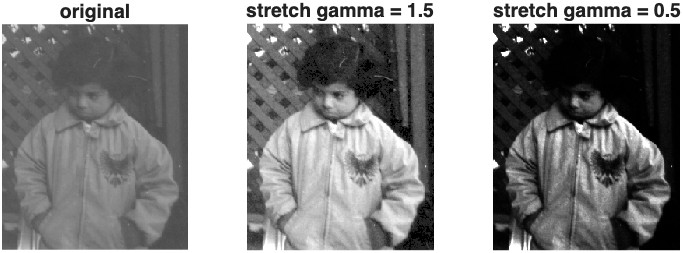
\includegraphics[width=0.6\textwidth]{lab4-gamma-pout-stretch.jpg}
  \caption{gamma correction with contrast stretch on pout.gif}\label{fig:l4-gamma-pout-stretch}
\end{figure}

TODO

\subsubsection{(b) as well with different pictures}

\begin{figure}[H]
  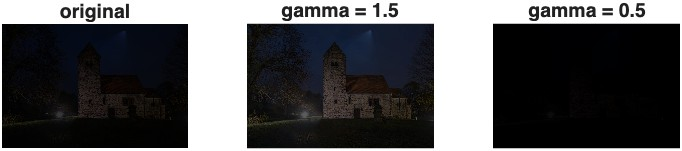
\includegraphics[width=0.6\textwidth]{lab4-gamma-church.jpg}
  \caption{gamma correction on church2.png}\label{fig:l4-gamma-church}
\end{figure}

\begin{figure}[H]
  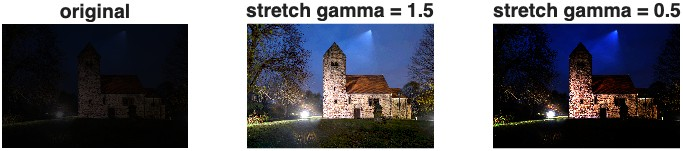
\includegraphics[width=0.6\textwidth]{lab4-gamma-church-stretch.jpg}
  \caption{gamma correction with contrast stretch on church2.png}\label{fig:l4-gamma-church-stretch}
\end{figure}

\begin{figure}[H]
  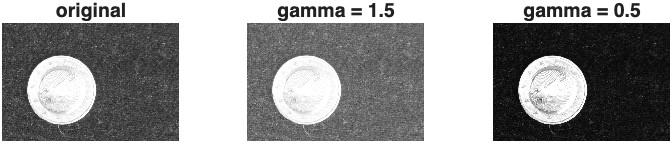
\includegraphics[width=0.6\textwidth]{lab4-gamma-adler.jpg}
  \caption{gamma correction on adler.jpg}\label{fig:l4-gamma-adler}
\end{figure}

\begin{figure}[H]
  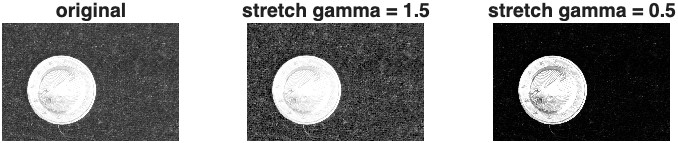
\includegraphics[width=0.6\textwidth]{lab4-gamma-adler-stretch.jpg}
  \caption{gamma correction with contrast stretch on adler.jpg}\label{fig:l4-gamma-adler-stretch}
\end{figure}

TODO

\subsection{Laboratory 4 -- Perform different techniques on lowandsp.gif}

\subsubsection{(a) to be finally able to highlight only the membranes and structures of the cells}

\begin{figure}[H]
  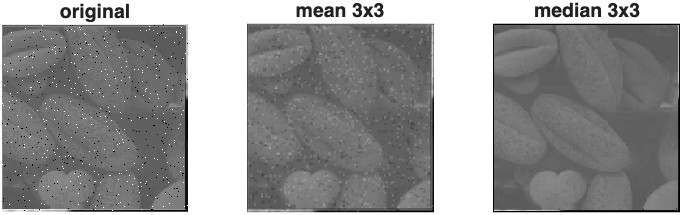
\includegraphics[width=0.6\textwidth]{lab4-cells-smoothing.jpg}
  \caption{original, mean filter, and median filter}\label{fig:l4-cells-smooth}
\end{figure}

\begin{figure}[H]
  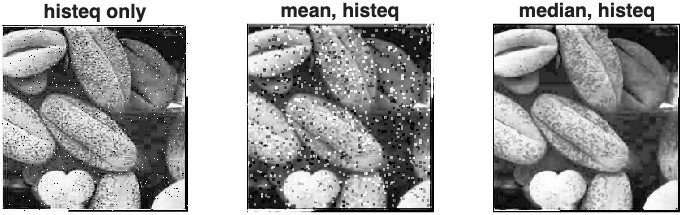
\includegraphics[width=0.6\textwidth]{lab4-cells-histeq.jpg}
  \caption{histogram equalization applied after filtering}\label{fig:l4-cells-histeq}
\end{figure}

\begin{figure}[H]
  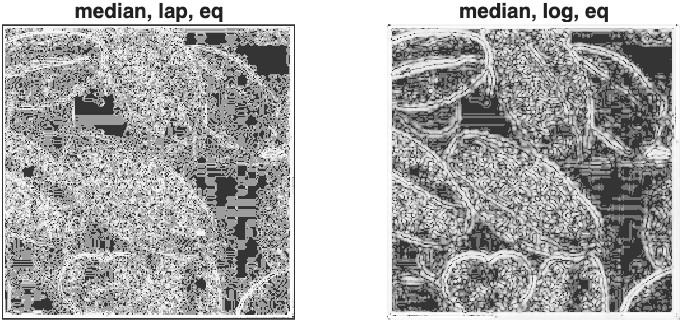
\includegraphics[width=0.48\textwidth]{lab4-cells-edges.jpg}
  \caption{edge detection with laplacian and LoG after equalization}\label{fig:l4-cells-edges}
\end{figure}

TODO

\subsection{Laboratory 4 -- Manipulate the following picture adler.jpg}

\subsubsection{(a) so that the background has only one colour without disturbing the coin}

TODO

\subsubsection{(b) so that the coin has only one colour without disturbing the background}

\begin{figure}[H]
  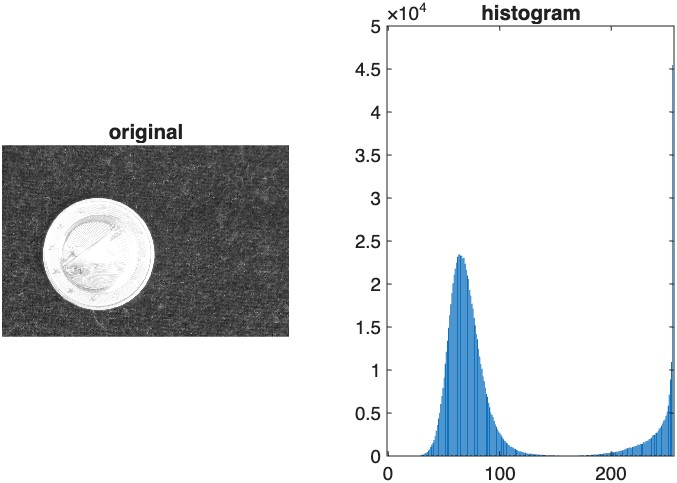
\includegraphics[width=0.6\textwidth]{lab4-adler-histogram.jpg}
  \caption{adler.jpg original and pixel histogram}\label{fig:l4-adler-hist}
\end{figure}

\begin{figure}[H]
  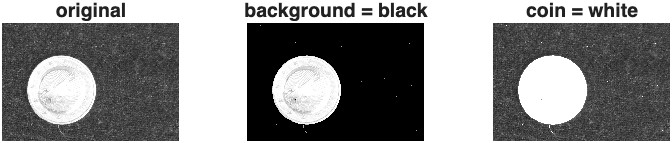
\includegraphics[width=0.6\textwidth]{lab4-adler-threshold.jpg}
  \caption{adler.jpg thresholding result}\label{fig:l4-adler-thresh}
\end{figure}

TODO

\subsection{Homework 4 (Diary only: Adapt your own histogram equalisation algorithm to perform a good result for the coloured picture church2.png)}

\begin{figure}[H]
  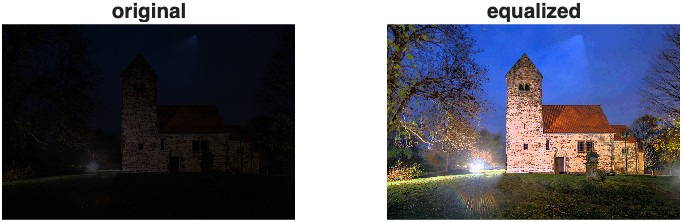
\includegraphics[width=0.6\textwidth]{hw4-hsv-equalization.jpg}
  \caption{HSV-based histogram equalization on church2.png}\label{fig:l4-hw4}
\end{figure}

TODO

% =====================================================================
%  LAB 5 -- Smoothing, Laplace, Unsharp Masking, GPU Challenge
%  Headings copied word for word from DSP2_Lab5_Exercise-2.pdf
%  NOTE: the Lab 5 sheet has no single topic line under "Lab Exercise",
%  so the chapter title below combines the four task titles -- rename it
%  if you prefer something else.
% =====================================================================
\clearpage
\section{Lab exercise 5: Smoothing and Noise Reduction, Edge Enhancement, Unsharp Masking, GPU Challenge}

TODO: chapter introduction -- theory about smoothing filters, Laplace
operator, unsharp masking and GPU computing.

\subsection{Laboratory 5 -- Smoothing and Noise Reduction}

% description given on the exercise sheet:
Smoothing filters are used to reduce noise, but they often result in blurring

\subsubsection{(a) Manual Implementation: Import the image 'cameraman.tif'. Implement a 3\hx3 Box Filter using only for loops. Each pixel should be replaced by the average of its 3\hx3 neighborhood.}

TODO

\subsubsection{(b) Comparison: Apply a 3\hx3 Gaussian Filter using the kernel G provided in the sources:}

% kernel given on the exercise sheet:
\[
  G = \frac{1}{16}
  \begin{pmatrix}
    1 & 2 & 1\\
    2 & 4 & 2\\
    1 & 2 & 1
  \end{pmatrix}
\]
Explain why the Gaussian filter results in less contour blurring than the Box filter.

TODO

\subsubsection{(c) Boundary Handling: Briefly describe how your code handles the edges of the image (e.g., zero-padding or ignoring borders).}

TODO

\subsection{Laboratory 5 -- Edge Enhancement with the Laplace Operator}

% description given on the exercise sheet:
The Laplace operator is used to highlight intensity changes by calculating the
second derivative.

\subsubsection{(a) Implementation: Apply the standard 3\hx3 Laplace kernel \texorpdfstring{$H_L$}{HL} to the Y (Luminance) component of the image 'peppers.png':}

% kernel given on the exercise sheet:
\[
  H_L =
  \begin{pmatrix}
    0 & 1 & 0\\
    1 & -4 & 1\\
    0 & 1 & 0
  \end{pmatrix}
\]
Use manual convolution (nested loops).

TODO

\subsubsection{(b) Visualization: The resulting image contains negative values. Explain how you visualize this ``Laplace image''correctly (e.g., using absolute values or shifting the zero-point).}

TODO

\subsection{Laboratory 5 -- Unsharp Masking}

% description given on the exercise sheet:
Unsharp masking enhances edges by subtracting a blurred version of the image
from the original

\subsubsection{(a) Calculation: Using your results from Task 1 and 2, implement a simple sharpening step: \texorpdfstring{$I_{sharp} = I_{original} - \mathrm{Laplace}(I_{original})$}{Isharp = Ioriginal - Laplace(Ioriginal)}.}

TODO

\subsubsection{(b) Effect: Describe the visual difference between the original image and the sharpened result.}

TODO

\subsection{Laboratory 5 -- GPU Challenge}

\subsubsection{(a) Benchmark a 5\hx5 convolution on a large image (e.g., 4000\hx4000) generated by the fractal.m. Compare the execution time of your nested for loops on the CPU versus the parallel execution on a GPU using gpuArray.}

% hints given on the exercise sheet:
\textbf{Hints for MATLAB GPU Implementation} To successfully complete the GPU
challenge, consider the following technical steps in MATLAB:
\begin{itemize}
  \item \textbf{Data Transfer:} Use the function \texttt{gpuArray(A)} to
        transfer a matrix from the CPU memory (RAM) to the GPU memory (VRAM).
  \item \textbf{Synchronization:} GPU operations are often asynchronous. To get
        an accurate measurement using \texttt{tic} and \texttt{toc}, you must
        call \texttt{wait(gpuDevice)} before stopping the timer to ensure all
        parallel threads have finished their execution.
  \item \textbf{Retrieval:} After the computation is complete, use the
        \texttt{gather(G)} function to move the result back to the CPU memory
        so it can be processed by standard functions like \texttt{imshow} or
        \texttt{imwrite}.
  \item \textbf{Compatibility:} You can check if a compatible hardware device
        is available by using the \texttt{gpuDeviceCount} function.
\end{itemize}

TODO

% =====================================================================
%  SOURCES  (same style as the DSP1 diary: a short prose paragraph)
% =====================================================================
\clearpage
\section{Sources}

% TODO: adjust this paragraph to the sources you actually used
As the main source of information, I have used the lecture script
Skript\_DSP\_3-0\_EN, and my notes made for the exam preparation based on
the lecture script. Also, internet articles for theory like Mathworks
mainly. I added a link to each source I referenced in the report text.

\clearpage
\section{Appendix}

The following images were provided as part of the lab exercise sheets
and used during the laboratory work.

\begin{figure}[H]
  \centering
  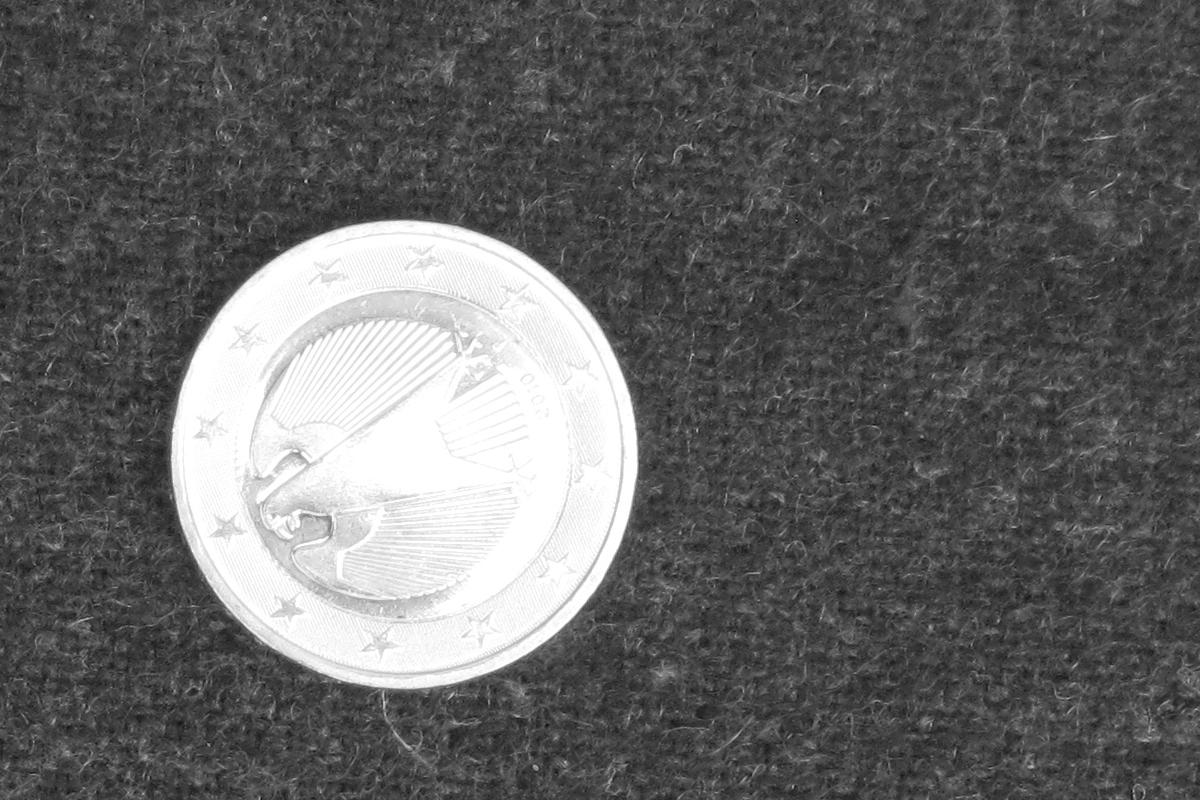
\includegraphics[width=0.45\textwidth]{adler.jpg}\hfill
  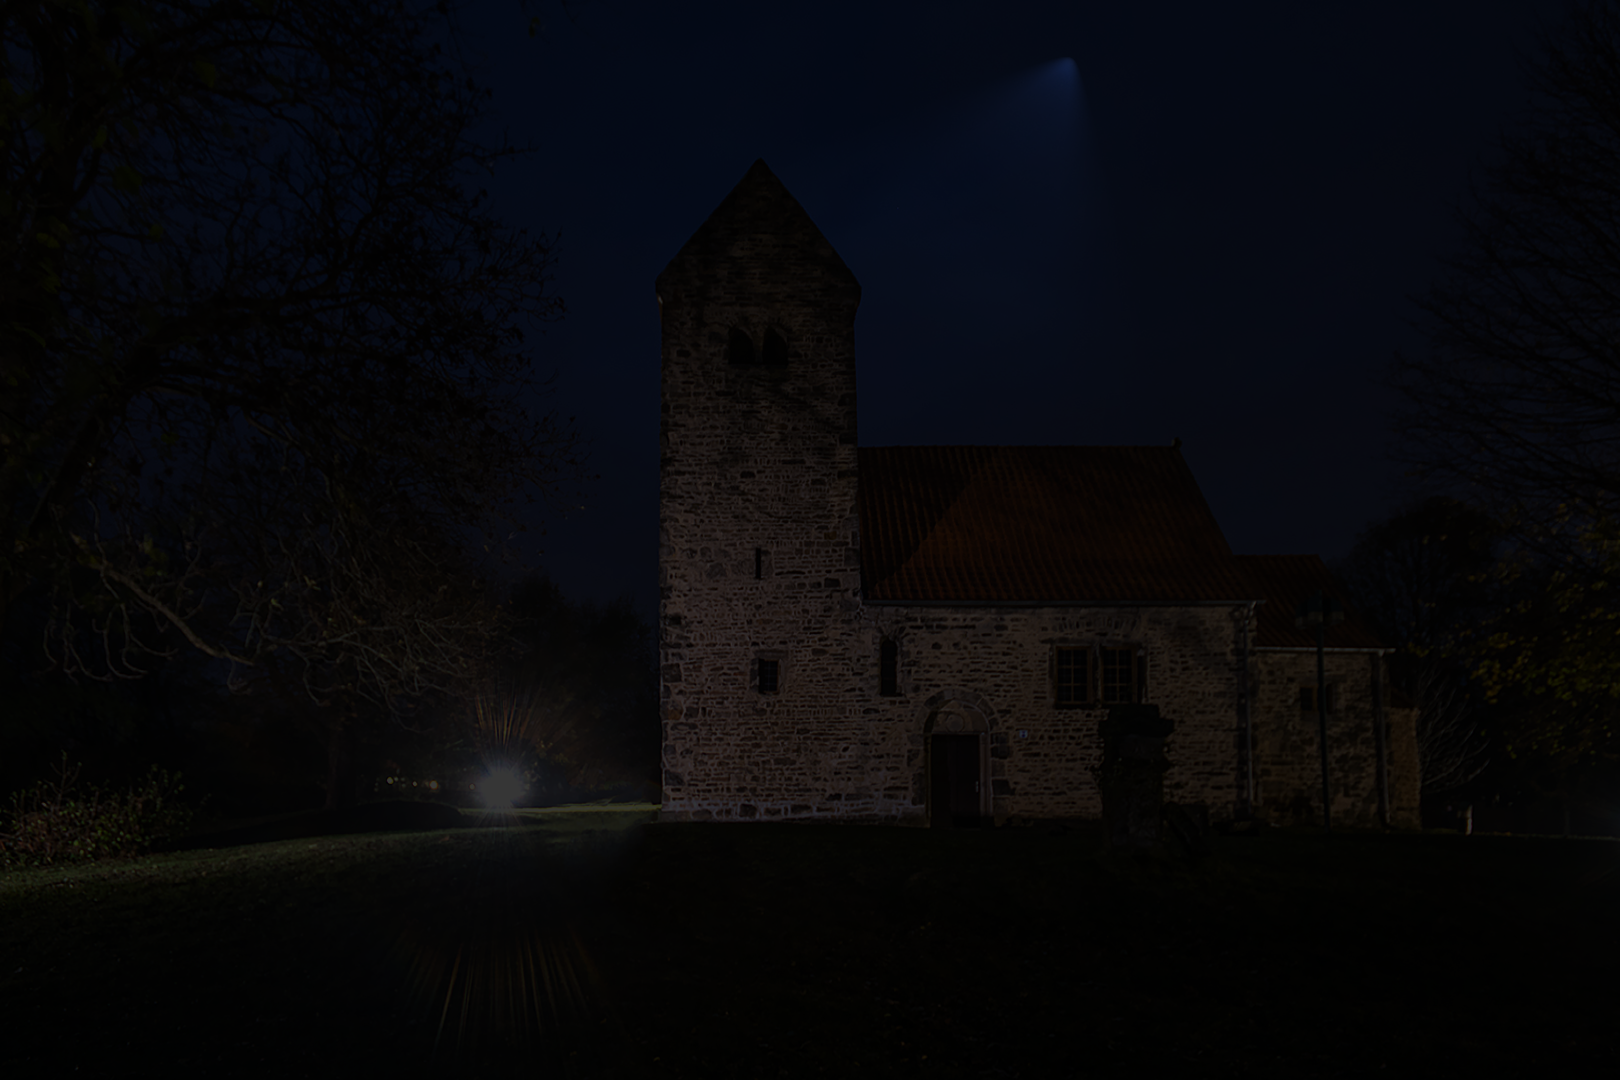
\includegraphics[width=0.45\textwidth]{church2.png}\\[8pt]
  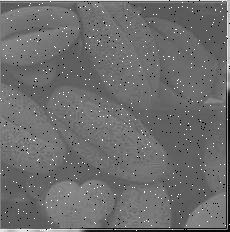
\includegraphics[width=0.45\textwidth]{lowandsp.png}\hfill
  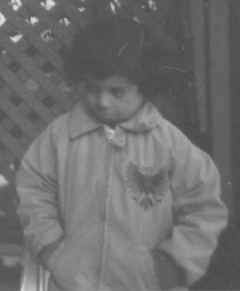
\includegraphics[width=0.45\textwidth]{pout.png}
  \caption{}\label{fig:app_resources}
\end{figure}


\end{document}
